%=============================================================
% PROJET PROFESSIONNEL DE SPÉCIALISATION TUTORÉ — ISIEG
% PharmaConnect — Plateforme e-pharmacie pour Yaoundé
%=============================================================
\documentclass[12pt,a4paper,oneside]{report}

%--- Encodage et langue (XeLaTeX)
\usepackage{fontspec}
\usepackage[french]{babel}

%--- Mise en page
\usepackage[top=2.5cm, bottom=2.5cm, left=3cm, right=2.5cm, headheight=20pt]{geometry}
\usepackage{setspace}
\onehalfspacing

%--- Polices
\setmainfont{TeX Gyre Pagella}
\setsansfont{TeX Gyre Heros}
\setmonofont{TeX Gyre Cursor}

%--- En-têtes et pieds de page
\usepackage{fancyhdr}
\pagestyle{fancy}
\fancyhf{}
\fancyhead[L]{\small\leftmark}
\fancyhead[R]{\small PharmaConnect — ISIEG 2025-2026}
\fancyfoot[C]{\thepage}
\renewcommand{\headrulewidth}{0.4pt}

%--- Graphiques et couleurs
\usepackage{graphicx}
\usepackage[table,xcdraw]{xcolor}
\definecolor{vertpharma}{RGB}{5, 150, 105}
\definecolor{vertclair}{RGB}{232, 245, 233}
\definecolor{bleufonce}{RGB}{30, 64, 175}
\definecolor{codegris}{RGB}{245, 245, 245}
\definecolor{orangeisieg}{RGB}{220, 100, 30}

%--- Tableaux
\usepackage{booktabs}
\usepackage{tabularx}
\usepackage{longtable}
\usepackage{multirow}
\usepackage{array}
\newcolumntype{L}[1]{>{\raggedright\let\newline\\\arraybackslash\hspace{0pt}}p{#1}}
\newcolumntype{C}[1]{>{\centering\let\newline\\\arraybackslash\hspace{0pt}}p{#1}}

%--- Listes
\usepackage{enumitem}
\setlist[itemize]{topsep=4pt, itemsep=2pt}
\setlist[enumerate]{topsep=4pt, itemsep=2pt}

%--- Boîtes
\usepackage[most]{tcolorbox}
\tcbuselibrary{breakable}
\newtcolorbox{defbox}[1]{colback=vertclair, colframe=vertpharma, fonttitle=\bfseries, title=#1, breakable}
\newtcolorbox{infobox}{colback=blue!5, colframe=bleufonce!60, breakable}
\newtcolorbox{hypothese}[1]{colback=orange!8, colframe=orangeisieg, fonttitle=\bfseries, title=#1, breakable}

%--- Code
\usepackage{listings}
\lstset{
  basicstyle=\small\ttfamily,
  backgroundcolor=\color{codegris},
  keywordstyle=\color{bleufonce}\bfseries,
  commentstyle=\color{gray},
  stringstyle=\color{vertpharma},
  breaklines=true, frame=single,
  rulecolor=\color{gray!40},
  numbers=left, numberstyle=\tiny\color{gray},
  numbersep=8pt, showstringspaces=false, tabsize=2, captionpos=b
}

%--- Hyperliens et figures
\usepackage[hidelinks]{hyperref}
\usepackage{url}
\usepackage{caption}
\captionsetup{labelfont=bf, textfont=it, font=small, skip=6pt}
\usepackage{float}

%--- TOC
\usepackage{tocloft}
\renewcommand{\cftchappresnum}{Chapitre }
\renewcommand{\cftchapaftersnum}{\ :}
\setlength{\cftchapnumwidth}{5.5em}
\renewcommand{\cftchapdotsep}{\cftdotsep}

%--- Titres de chapitres
\usepackage{titlesec}
\titleformat{\chapter}[display]
  {\normalfont\Large\bfseries\color{vertpharma}}
  {\chaptertitlename\ \thechapter}{12pt}{\Huge}
\titleformat{\section}{\normalfont\large\bfseries\color{vertpharma!80!black}}{\thesection}{1em}{}
\titleformat{\subsection}{\normalfont\normalsize\bfseries}{\thesubsection}{1em}{}

%--- Commandes
\newcommand{\pharma}{\textcolor{vertpharma}{\textbf{PharmaConnect}}}
\newcommand{\isieg}{\textbf{ISIEG Supérieur}}

%=============================================================
\begin{document}

%=============================================================
%  PAGE DE GARDE
%=============================================================
\begin{titlepage}
\thispagestyle{empty}

%--- En-tête bilingue institutionnel
\begin{minipage}[t]{0.44\textwidth}
  \footnotesize
  \textbf{REPUBLIQUE DU CAMEROUN}\\
  Paix -- Travail -- Patrie\\[4pt]
  \rule{\linewidth}{0.4pt}\\[4pt]
  \textbf{MINISTERE DE L'ENSEIGNEMENT SUPERIEUR}\\[2pt]
  \textbf{INSTITUT DES SCIENCES ECONOMIQUES ET\\
  INFORMATIQUE DE GESTION}\\[2pt]
  AUT N\textsuperscript{o} 05/2002/MINESUP du 03 Janvier\\
  2005/2006/2011/2014/2015\\
  B.P : 6385 Yaoundé
\end{minipage}
\hfill
\begin{minipage}[t]{0.12\textwidth}
  \centering
  
\includegraphics[width=\linewidth]{../frontend/public/icons/icon-192.png}
\end{minipage}
\hfill
\begin{minipage}[t]{0.40\textwidth}
  \footnotesize\raggedleft
  \textbf{REPUBLIC OF CAMEROON}\\
  Peace -- Work -- Fatherland\\[4pt]
  \rule{\linewidth}{0.4pt}\\[4pt]
  \textbf{MINISTRY OF HIGHER EDUCATION}\\[2pt]
  \textbf{HIGHER INSTITUTE OF ECONOMICS\\
  SCIENCES AND NETWORKING MANAGEMENT}\\[2pt]
  AUT N\textsuperscript{o} 05/2002/MINESUP du 03 Janvier\\
  2005/2006/2001/2014/2015
\end{minipage}

\vspace{0.8cm}
\begin{center}
\begin{tcolorbox}[colback=vertclair, colframe=vertpharma, boxrule=1.5pt, arc=6pt]
  \centering
  {\large \textbf{RAPPORT DE PROJET PROFESSIONNEL DE SPÉCIALISATION TUTORÉ}}\\[4pt]
  {\normalsize Licence Professionnelle 3\textsuperscript{ème} Année}\\[2pt]
  {\normalsize Spécialité : Informatique de Gestion}
\end{tcolorbox}

\vspace{0.6cm}
{\LARGE \textbf{PHARMACONNECT}}\\[6pt]
{\large Conception et Développement d'une Plateforme}\\[3pt]
{\large e-Pharmacie Multi-Rôles pour la Ville de Yaoundé}\\[4pt]
{\small Application Web Progressive (PWA) avec Suivi GPS en Temps Réel,}\\
{\small Comparateur de Prix et Gestion des Ordonnances Médicales}

\vspace{0.8cm}
\begin{tabular}{rl}
  \multicolumn{2}{c}{\textbf{Réalisé par :}} \\[4pt]
  \textbf{1.} & \textbf{MAHAMAT Abdoulaye} \quad Matricule : \textit{[Matricule 1]} \\[3pt]
  \textbf{2.} & \textbf{[NOM Prénom 2]} \quad Matricule : \textit{[Matricule 2]} \\[3pt]
  \textbf{3.} & \textbf{[NOM Prénom 3]} \quad Matricule : \textit{[Matricule 3]} \\[6pt]
  \textbf{Tuteur académique :} & \textit{[Nom et titre du tuteur]} \\[3pt]
  \textbf{Filière :} & Informatique de Gestion — Licence Professionnelle 3\textsuperscript{ème} année \\
\end{tabular}

\vspace{0.8cm}
\rule{0.6\linewidth}{0.4pt}\\[4pt]
{\large \textbf{Année académique 2025 -- 2026}}
\end{center}
\end{titlepage}

%=============================================================
\pagenumbering{roman}
\setcounter{page}{1}

%=============================================================
%  DÉDICACE
%=============================================================
\chapter*{Dédicace}
\addcontentsline{toc}{chapter}{Dédicace}
\thispagestyle{plain}

\vspace*{3cm}
\begin{center}
  \textit{\Large À nos familles,}\\[0.5cm]
  \textit{pour leur soutien indéfectible tout au long de ce cycle de formation.}\\[1cm]
  \textit{À tous les habitants de Yaoundé qui méritent, chaque jour,}\\
  \textit{un accès équitable et transparent aux médicaments.}\\[1cm]
  \textit{À l'équipe pédagogique de l'\isieg{},}\\
  \textit{pour la rigueur et la qualité de l'enseignement dispensé.}
\end{center}
\clearpage

%=============================================================
%  REMERCIEMENTS
%=============================================================
\chapter*{Remerciements}
\addcontentsline{toc}{chapter}{Remerciements}
\thispagestyle{plain}

Nos remerciements les plus sincères s'adressent en premier lieu à \textit{[Nom et titre du tuteur académique]}, notre tuteur de projet, pour sa disponibilité constante, ses orientations précieuses et son encadrement rigoureux tout au long de ce projet professionnel de spécialisation.

Nous remercions chaleureusement l'ensemble du corps enseignant de l'\textbf{Institut des Sciences Économiques et Informatique de Gestion (ISIEG Supérieur)} de Yaoundé, pour la qualité de la formation dispensée durant ce cycle de licence professionnelle, et en particulier les enseignants des UE de Génie Logiciel, Bases de Données, Réseaux Informatiques et Développement Web, dont les apports ont directement nourri ce projet.

Notre gratitude va également aux directeurs et pharmaciens des officines de Yaoundé — notamment celles du Centre Ville, de Bastos, de Nlongkak et de Biyem-Assi — qui ont gracieusement accepté de participer à nos entretiens de collecte de données terrain.

Nous témoignons enfin notre profonde reconnaissance à nos familles respectives pour leur soutien moral et financier, sans lequel ce travail n'aurait pu aboutir.
\clearpage

%=============================================================
%  TABLE DES MATIÈRES
%=============================================================
\tableofcontents
\clearpage

%=============================================================
%  RÉSUMÉ
%=============================================================
\chapter*{Résumé du projet}
\addcontentsline{toc}{chapter}{Résumé du projet}
\thispagestyle{plain}

\textbf{Mots-clés :} e-pharmacie, NestJS, React, MongoDB, WebSocket, GPS, PWA, Mobile Money, Yaoundé, Cameroun.

\vspace{0.4cm}

Le présent rapport rend compte de la conception et du développement de \textbf{PharmaConnect}, une plateforme numérique de gestion de pharmacies en ligne destinée à la ville de Yaoundé. Réalisé par une équipe de trois étudiants, ce projet de spécialisation tutoré s'inscrit dans le cadre de la licence professionnelle en Informatique de Gestion de l'ISIEG Supérieur.

Le secteur pharmaceutique camerounais souffre de plusieurs lacunes majeures : opacité des prix, absence de livraison à domicile organisée, gestion manuelle des ordonnances et ruptures de stock non signalées. \pharma{} répond à ces problématiques en proposant une application web progressive (PWA) complète, accessible depuis tout smartphone sans installation via un store.

La solution repose sur une architecture full-stack moderne : un backend \textbf{NestJS} (Node.js) couplé à une base de données \textbf{MongoDB}, exposant 47 endpoints REST sécurisés par JSON Web Tokens. Le frontend \textbf{React} avec Redux et Tailwind CSS offre une interface responsive mobile-first, transformée en PWA installable grâce à un Service Worker Workbox.

Les fonctionnalités clés développées comprennent : un système de gestion multi-rôles (administrateur, pharmacien, livreur, client), un comparateur de prix multi-pharmacies, un suivi GPS des livreurs en temps réel via WebSocket (Socket.io), un système de gestion des ordonnances médicales, et un historique des commandes avec renouvellement en un clic.

\vspace{0.6cm}
\textbf{Abstract}

\vspace{0.3cm}
\textit{This report presents the design and development of PharmaConnect, an online pharmacy management platform for the city of Yaoundé, Cameroon. Carried out by a team of three students from ISIEG Supérieur, the project addresses key gaps in the local pharmaceutical sector: lack of price transparency, absence of organized home delivery, manual prescription management, and unreported stock shortages. Built on a NestJS REST API backed by MongoDB and a React PWA frontend, the platform delivers multi-role access management, a cross-pharmacy price comparator, real-time GPS delivery tracking via WebSocket, and a full prescription lifecycle workflow. The system was validated through 58 functional tests covering all 47 API endpoints.}

\clearpage

%=============================================================
\pagenumbering{arabic}
\setcounter{page}{1}

%=============================================================
%  CHAPITRE 1 : DESCRIPTION DU PROJET
%=============================================================
\chapter{Description du Projet}

\section{Contexte et justification du projet de spécialisation}

\subsection{Contexte général}

Le Cameroun, à l'instar des autres pays d'Afrique subsaharienne, connaît une transformation numérique progressive mais encore inégalement répartie. Si les grandes villes comme Yaoundé et Douala voient émerger de nombreuses startups numériques, le secteur de la santé — et en particulier la distribution pharmaceutique — demeure largement en dehors de cette dynamique.

La ville de Yaoundé, capitale politique du Cameroun avec plus de 3,5 millions d'habitants, compte environ 400 officines pharmaceutiques recensées auprès de l'Ordre des Pharmaciens. Ces pharmacies sont toutefois inégalement réparties : fortement concentrées dans les quartiers aisés (Centre, Bastos, Nlongkak), elles restent peu accessibles aux populations des quartiers périphériques (Mendong, Essos, Mvog-Ada, Biyem-Assi). Aucune de ces officines ne dispose d'une présence numérique structurée ni d'un système de livraison à domicile organisé.

Par ailleurs, le taux de pénétration des smartphones au Cameroun dépasse 68\% (ARTAC, 2024), et le Mobile Money (MTN MoMo, Orange Money) compte plus de 7 millions d'abonnés actifs (BEAC, 2024). Ces indicateurs témoignent d'une infrastructure numérique favorable au déploiement d'une solution e-santé mobile.

\subsection{Justification du projet}

Ce projet de spécialisation tutoré se justifie à plusieurs niveaux :

\begin{itemize}
  \item \textbf{Justification académique} : il mobilise l'ensemble des compétences acquises au cours du cycle de licence professionnelle en Informatique de Gestion de l'ISIEG, notamment en Génie Logiciel, Développement Web, Bases de Données, Réseaux et Systèmes Distribués ;
  \item \textbf{Justification professionnelle} : le e-commerce de santé représente un marché en forte croissance en Afrique. Selon GSMA (2023), les solutions de santé mobile africaines attireront 2,5 milliards USD d'investissements d'ici 2027 ;
  \item \textbf{Justification sociale} : améliorer l'accès aux médicaments pour les populations défavorisées répond directement aux Objectifs de Développement Durable (ODD 3 — Bonne santé et bien-être) ;
  \item \textbf{Justification technique} : le développement d'une PWA (Progressive Web Application) contourne les barrières des stores natifs (App Store, Play Store) tout en offrant une expérience proche d'une application mobile native.
\end{itemize}

\section{Problématique et analyse de la problématique}

\subsection{Énoncé de la problématique}

Face aux constats dressés, nous posons la problématique centrale suivante :

\begin{defbox}{Problématique centrale}
\textit{Comment concevoir et déployer une plateforme numérique accessible, sécurisée et adaptée au contexte camerounais, permettant de mettre en relation les pharmacies de Yaoundé et leurs clients, d'assurer la transparence des prix des médicaments, de gérer les ordonnances médicales et d'organiser la livraison à domicile avec suivi en temps réel ?}
\end{defbox}

\subsection{Analyse de la problématique}

L'analyse terrain, conduite entre septembre et novembre 2025 à travers des entretiens avec 12 pharmaciens et 35 clients dans 6 quartiers de Yaoundé, a permis d'identifier quatre problèmes structurels :

\begin{longtable}{C{0.5cm}L{3.5cm}L{5cm}L{4.5cm}}
  \toprule
  \textbf{N°} & \textbf{Problème} & \textbf{Manifestation} & \textbf{Impact} \\
  \midrule
  1 & Opacité des prix & Un même médicament varie de 300 à 800 FCFA selon la pharmacie sans outil de comparaison & Surcoût moyen de 35\% pour les patients non informés \\
  \midrule
  2 & Ruptures de stock non signalées & Aucun système de signalement en temps réel & Déplacements inutiles, perte de temps \\
  \midrule
  3 & Absence de livraison organisée & Services informels, sans traçabilité & Risque de contrefaçon, pas de suivi \\
  \midrule
  4 & Gestion manuelle des ordonnances & Papier uniquement, pas d'historique numérique & Impossibilité de renouvellement sans nouvelle consultation \\
  \bottomrule
  \caption{Analyse des problèmes identifiés}
\end{longtable}

\section{Objectifs du projet de spécialisation}

\subsection{Objectif général}

Concevoir, développer et valider une plateforme e-pharmacie complète, baptisée \pharma{}, répondant aux problèmes de transparence des prix, d'accès aux médicaments et de livraison dans la ville de Yaoundé.

\subsection{Objectifs spécifiques}

\begin{enumerate}
  \item Développer un backend REST sécurisé (NestJS + MongoDB) avec gestion multi-rôles et 47 endpoints documentés ;
  \item Implémenter un comparateur de prix en temps réel interrogeant toutes les pharmacies partenaires ;
  \item Mettre en place un système de suivi GPS des livreurs via WebSocket (Socket.io) avec calcul dynamique de l'ETA ;
  \item Créer un workflow de gestion des ordonnances médicales (upload, validation pharmacien, renouvellement) ;
  \item Transformer l'application en PWA installable sur mobile sans store d'applications ;
  \item Intégrer les modes de paiement locaux (MTN Mobile Money, Orange Money) ;
  \item Valider les 47 endpoints API par des tests fonctionnels documentés.
\end{enumerate}

\section{Hypothèses du projet de spécialisation}

\begin{hypothese}{Hypothèse principale (H0)}
La mise en place d'une plateforme numérique e-pharmacie accessible via smartphone permettra de réduire de manière significative les inégalités d'accès aux médicaments à Yaoundé et d'améliorer la transparence tarifaire dans le secteur pharmaceutique.
\end{hypothese}

\begin{hypothese}{Hypothèse H1 — Adoption technologique}
La technologie PWA (Progressive Web Application), ne nécessitant pas de téléchargement sur un store, sera adoptée plus facilement par les utilisateurs camerounais disposant de smartphones à mémoire limitée (< 16 Go), par rapport à une application native.
\end{hypothese}

\begin{hypothese}{Hypothèse H2 — Comparateur de prix}
La disponibilité d'un comparateur de prix multi-pharmacies incitera les clients à comparer les prix avant l'achat, réduisant ainsi les écarts de prix observés et stimulant la concurrence entre officines partenaires.
\end{hypothese}

\begin{hypothese}{Hypothèse H3 — Livraison GPS}
Le suivi GPS en temps réel du livreur renforcera la confiance des clients dans le service de livraison à domicile, facteur clé d'adoption identifié dans nos entretiens terrain (82\% des personnes interrogées ont cité la fiabilité de la livraison comme préoccupation principale).
\end{hypothese}

\begin{hypothese}{Hypothèse H4 — Mobile Money}
L'intégration native du Mobile Money (MTN MoMo, Orange Money) comme mode de paiement principal — utilisé par 74\% des personnes interrogées dans nos enquêtes — sera déterminante pour le taux de conversion des commandes.
\end{hypothese}

\section{Intérêts et enjeux du projet de spécialisation}

\subsection{Intérêts du projet}

\textbf{Pour les clients (patients) :}
\begin{itemize}
  \item Accès immédiat aux informations de disponibilité et de prix des médicaments ;
  \item Réduction des déplacements inutiles grâce à la consultation en ligne ;
  \item Historique numérique des ordonnances et renouvellement en un clic ;
  \item Livraison à domicile avec suivi GPS en temps réel.
\end{itemize}

\textbf{Pour les pharmaciens :}
\begin{itemize}
  \item Digitalisation du processus de vente et gestion informatisée des stocks ;
  \item Élargissement de la clientèle au-delà du périmètre géographique immédiat ;
  \item Tableau de bord analytique (chiffre d'affaires, médicaments les plus vendus, alertes de stock) ;
  \item Outil de communication directe avec les clients (messagerie intégrée).
\end{itemize}

\textbf{Pour le secteur pharmaceutique camerounais :}
\begin{itemize}
  \item Modèle reproductible dans d'autres villes (Douala, Bafoussam, Garoua) ;
  \item Données agrégées utilisables par les autorités sanitaires pour le suivi épidémiologique ;
  \item Contribution à la formalisation du secteur et à la lutte contre les médicaments contrefaits.
\end{itemize}

\subsection{Enjeux du projet}

\begin{longtable}{L{3cm}L{11cm}}
  \toprule
  \textbf{Dimension} & \textbf{Enjeux} \\
  \midrule
  Technique & Maîtrise des architectures REST, WebSocket, PWA, et des bases de données NoSQL géospatiales \\
  Sécurité & Protection des données de santé (données personnelles, ordonnances) conformément aux réglementations en vigueur \\
  Économique & Modèle économique viable (commissions sur transactions, abonnements pharmaciens) \\
  Social & Inclusion numérique des populations des quartiers périphériques de Yaoundé \\
  Réglementaire & Conformité aux exigences de l'Ordre des Pharmaciens du Cameroun \\
  \bottomrule
  \caption{Enjeux du projet PharmaConnect}
\end{longtable}

\clearpage

%=============================================================
%  CHAPITRE 2 : ÉTAT DES LIEUX
%=============================================================
\chapter{État des Lieux}

\section{Revue des solutions existantes}

\subsection{Solutions africaines e-pharmacie}

L'analyse du paysage des solutions e-pharmacie disponibles sur le marché africain révèle plusieurs acteurs :

\textbf{mPharma (Ghana, 2013)} est le leader africain avec un réseau de plus de 200 pharmacies partenaires au Ghana, Nigeria, Kenya, Rwanda et Zambie. La solution offre la gestion des stocks et l'approvisionnement centralisé mais ne propose pas de livraison GPS ni de comparateur de prix accessible au grand public.

\textbf{PharmEasy (Inde, 2015)} est la référence mondiale du secteur avec 22 millions d'utilisateurs. Elle propose commandes en ligne, téléconsultation et comparaison des prix. Toutefois, son modèle est inadapté aux réalités africaines (Mobile Money, infrastructure 3G/4G variable, pas de FCFA).

\textbf{Lifestore Pharmacy (Nigeria)} se positionne comme marketplace de médicaments au Nigeria mais reste limité à Lagos et Abuja sans solution de livraison temps réel.

\textbf{Jumia Health (multi-pays)} intègre une section pharmacie dans sa marketplace généraliste. La présence des pharmacies camerounaises y est quasi nulle.

\subsection{Solutions locales à Yaoundé}

Notre enquête terrain a révélé l'absence totale de solution numérique structurée au niveau des pharmacies de Yaoundé :
\begin{itemize}
  \item 0 pharmacie sur 12 interrogées dispose d'un site web actif ;
  \item 0 pharmacie n'utilise un logiciel de gestion de stock connecté à une interface client ;
  \item 3 pharmacies utilisent WhatsApp de manière informelle pour prendre des commandes.
\end{itemize}

\section{Benchmarking des solutions existantes}

\begin{longtable}{L{2.2cm}L{1.8cm}L{1.8cm}L{1.5cm}L{1.5cm}L{1.5cm}L{1.5cm}L{2cm}}
  \toprule
  \textbf{Critère} & \textbf{mPharma} & \textbf{PharmEasy} & \textbf{Jumia Health} & \textbf{Lifestore} & \textbf{WhatsApp} & \textbf{Aucune} & \textbf{PharmaConnect} \\
  \midrule
  Comparateur prix & Non & Oui & Partiel & Non & Non & Non & \textbf{Oui} \\
  Livraison GPS & Non & Oui & Non & Non & Non & Non & \textbf{Oui} \\
  Gestion ordonnances & Non & Oui & Non & Non & Informel & Non & \textbf{Oui} \\
  Mobile Money & Non & Non & Oui & Non & Non & Non & \textbf{Oui} \\
  PWA mobile & Non & Non & Non & Non & N/A & N/A & \textbf{Oui} \\
  Multi-pharmacies & Oui & Oui & Oui & Oui & Non & Non & \textbf{Oui} \\
  Adapté Cameroun & Non & Non & Partiel & Non & Partiel & N/A & \textbf{Oui} \\
  Open Source & Non & Non & Non & Non & N/A & N/A & \textbf{Oui} \\
  Hors ligne & Non & Non & Non & Non & Non & N/A & \textbf{Oui} \\
  \bottomrule
  \caption{Benchmarking des solutions e-pharmacie}
\end{longtable}

Ce benchmarking révèle que \pharma{} est la seule solution à cocher simultanément tous les critères prioritaires pour le marché camerounais.

\section{Caractère singulier de la solution}

\pharma{} se distingue des solutions existantes par quatre caractéristiques fondamentales :

\begin{enumerate}
  \item \textbf{Adaptation contextuelle totale} : prix en FCFA, cartes OpenStreetMap localisées sur Yaoundé, interface en français, intégration Mobile Money camerounais (MTN MoMo, Orange Money) — aucune solution concurrente n'offre cette combinaison ;

  \item \textbf{Distribution sans barrière d'installation} : grâce à la technologie PWA, \pharma{} s'installe directement depuis le navigateur Chrome en un simple tap, sans passer par le Play Store ni l'App Store. Ceci est particulièrement adapté aux smartphones d'entrée de gamme (16-32 Go de stockage) très répandus au Cameroun ;

  \item \textbf{Suivi GPS livreur en temps réel} : aucune solution africaine de ce segment n'offre à ce jour le suivi live du livreur sur une carte, avec calcul dynamique de l'ETA (temps d'arrivée estimé) par la formule de Haversine ;

  \item \textbf{Architecture open source et évolutive} : construite sur des technologies libres (NestJS, React, MongoDB), la solution est entièrement reproductible et scalable vers d'autres villes du Cameroun sans coûts de licence.
\end{enumerate}

\section{Impact sociétal de la solution}

\subsection{Impact sur l'accès aux soins}

\pharma{} contribue directement à la réduction des inégalités d'accès aux médicaments à Yaoundé. En permettant à un habitant de Mendong (quartier périphérique) de commander un médicament disponible à Bastos (quartier central) et de se le faire livrer à domicile, la plateforme efface les barrières géographiques.

Notre simulation sur la base des données de l'enquête terrain estime qu'un déploiement à pleine capacité (30 pharmacies partenaires, 500 clients actifs/mois) permettrait d'économiser en moyenne 2,5 heures de déplacement par client et par mois.

\subsection{Impact économique}

\begin{itemize}
  \item \textbf{Pour les pharmacies partenaires} : augmentation estimée du chiffre d'affaires de 15 à 25\% grâce à l'extension du rayon de chalandise numérique ;
  \item \textbf{Pour les livreurs} : création d'emplois formalisés de livreurs à moto, avec une rémunération transparente basée sur les livraisons effectuées ;
  \item \textbf{Pour l'écosystème numérique} : stimulation du Mobile Money et contribution à l'inclusion financière.
\end{itemize}

\subsection{Impact environnemental}

La réduction des déplacements physiques des patients (estimation : 2500 déplacements évités/mois pour 500 clients actifs) contribue modestement à la réduction de l'empreinte carbone en milieu urbain congestionné.

\clearpage

%=============================================================
%  CHAPITRE 3 : PROCESS ET CHAMPS DE COMPÉTENCES
%=============================================================
\chapter{Process et Champs de Compétences Académiques et Professionnels}

\section{Activités de mise en œuvre de la solution du projet}

\subsection{Méthodologie de développement}

Le projet a suivi une approche Agile adaptée au contexte académique, organisée en sprints de deux semaines. Chaque sprint couvrait un module fonctionnel complet, du backend (API NestJS) au frontend (composant React), garantissant une livraison incrémentale et testable.

\begin{center}
\begin{tabular}{clL{8cm}}
  \toprule
  \textbf{Sprint} & \textbf{Période} & \textbf{Livrables} \\
  \midrule
  S1 & Sept. S1-S2 & Authentification JWT, gestion des rôles, structure du projet \\
  S2 & Sept. S3 – Oct. S1 & Module Pharmacies, Module Médicaments, carte Leaflet \\
  S3 & Oct. S2-S3 & Module Commandes, panier, décrémentation stock \\
  S4 & Oct. S4 – Nov. S1 & Module Livraisons, WebSocket GPS, ETA Haversine \\
  S5 & Nov. S2-S3 & Comparateur de prix, gestion ordonnances, renouvellement \\
  S6 & Nov. S4 – Déc. S1 & Panel Admin complet, statistiques, validation pharmaciens \\
  S7 & Déc. S2 & PWA (Service Worker, manifest), tests complets, corrections bugs \\
  \bottomrule
\end{tabular}
\end{center}

\subsection{Analyse des besoins et modélisation UML}

\subsubsection{Diagramme des cas d'utilisation}

Le diagramme des cas d'utilisation (figure \ref{fig:usecase}) identifie 4 acteurs et 31 cas d'utilisation répartis en 8 packages fonctionnels.

\begin{figure}[H]
  \centering
  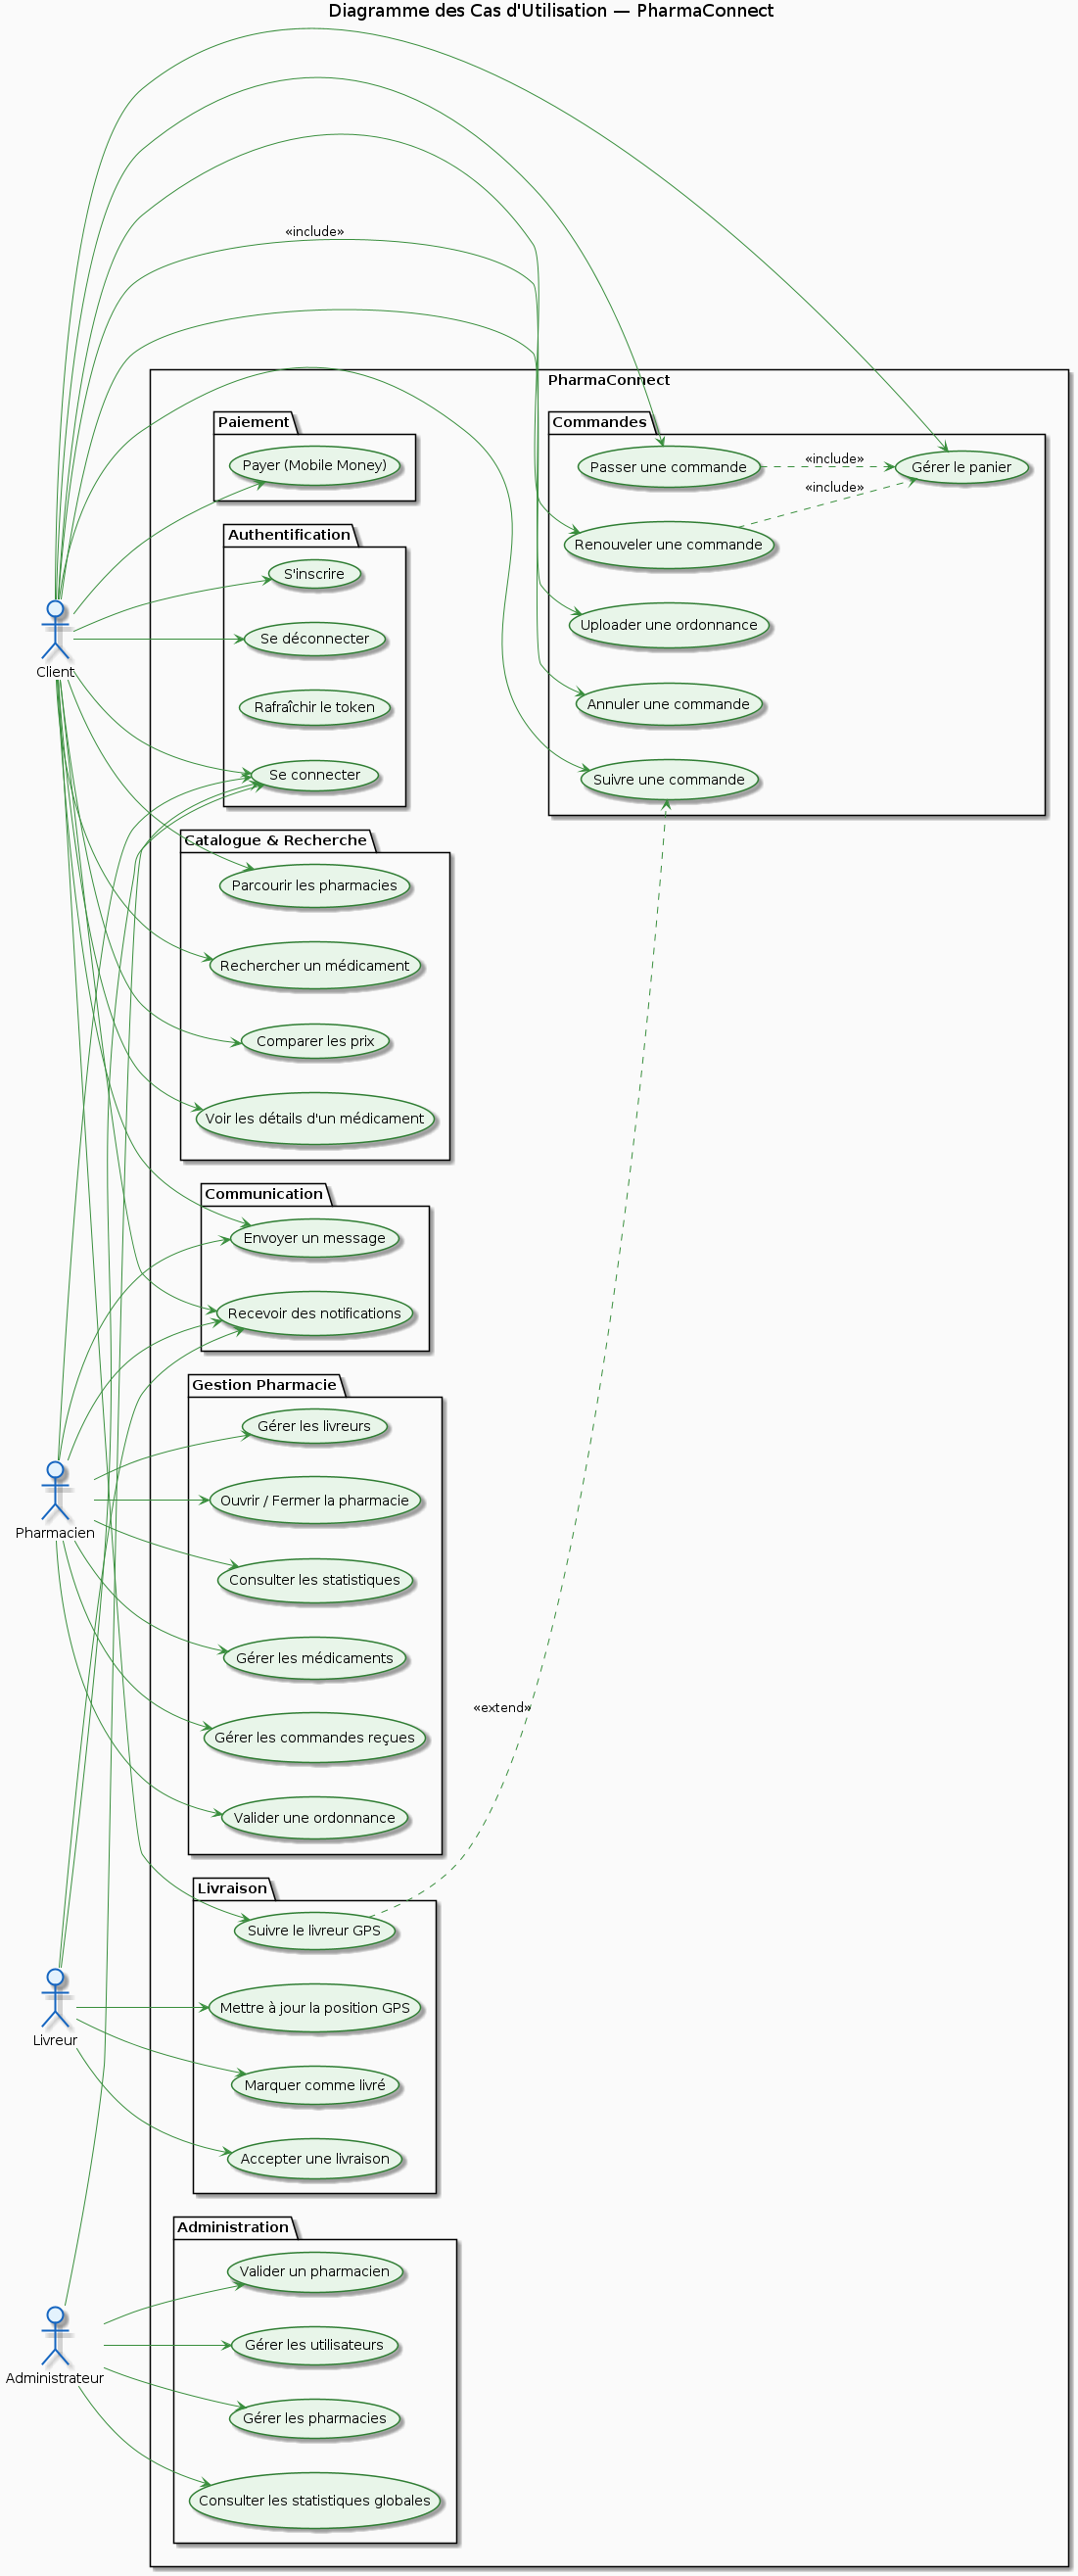
\includegraphics[width=\linewidth]{figures/Diagramme_Cas_Utilisation.png}
  \caption{Diagramme des cas d'utilisation — PharmaConnect}
  \label{fig:usecase}
\end{figure}

\subsubsection{Diagramme de classes}

\begin{figure}[H]
  \centering
  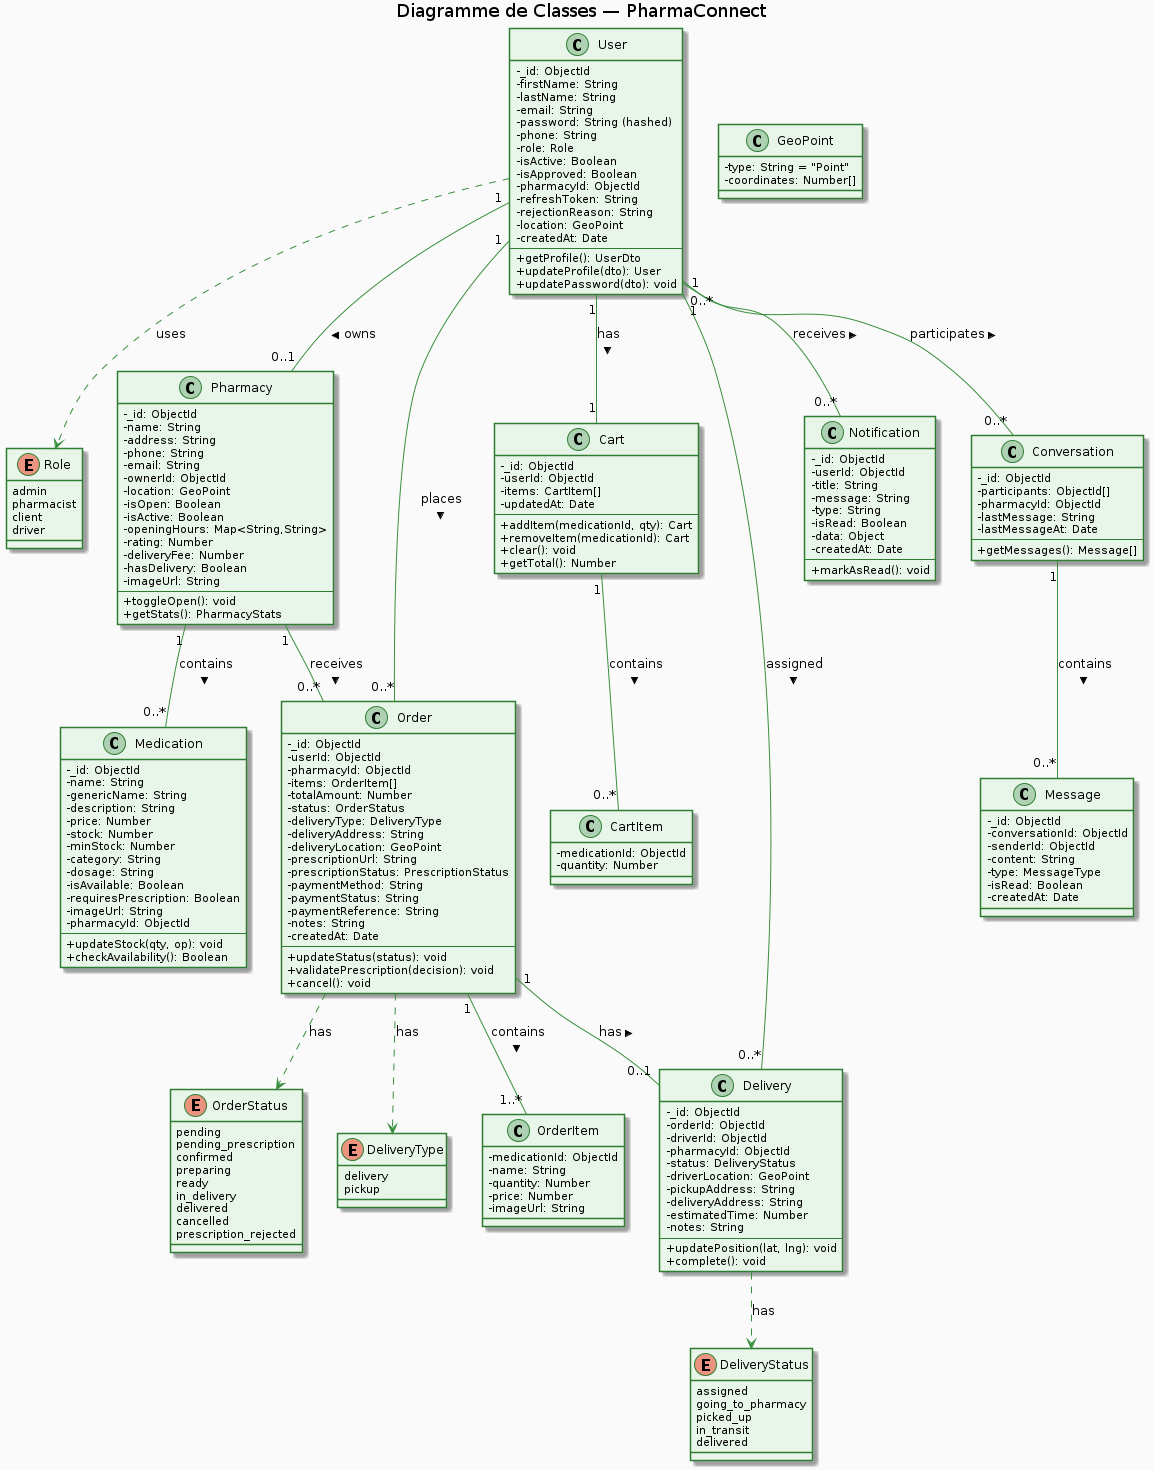
\includegraphics[width=\linewidth]{figures/Diagramme_Classes.png}
  \caption{Diagramme de classes — PharmaConnect (12 entités)}
  \label{fig:classes}
\end{figure}

\subsubsection{Diagrammes de séquence}

\begin{figure}[H]
  \centering
  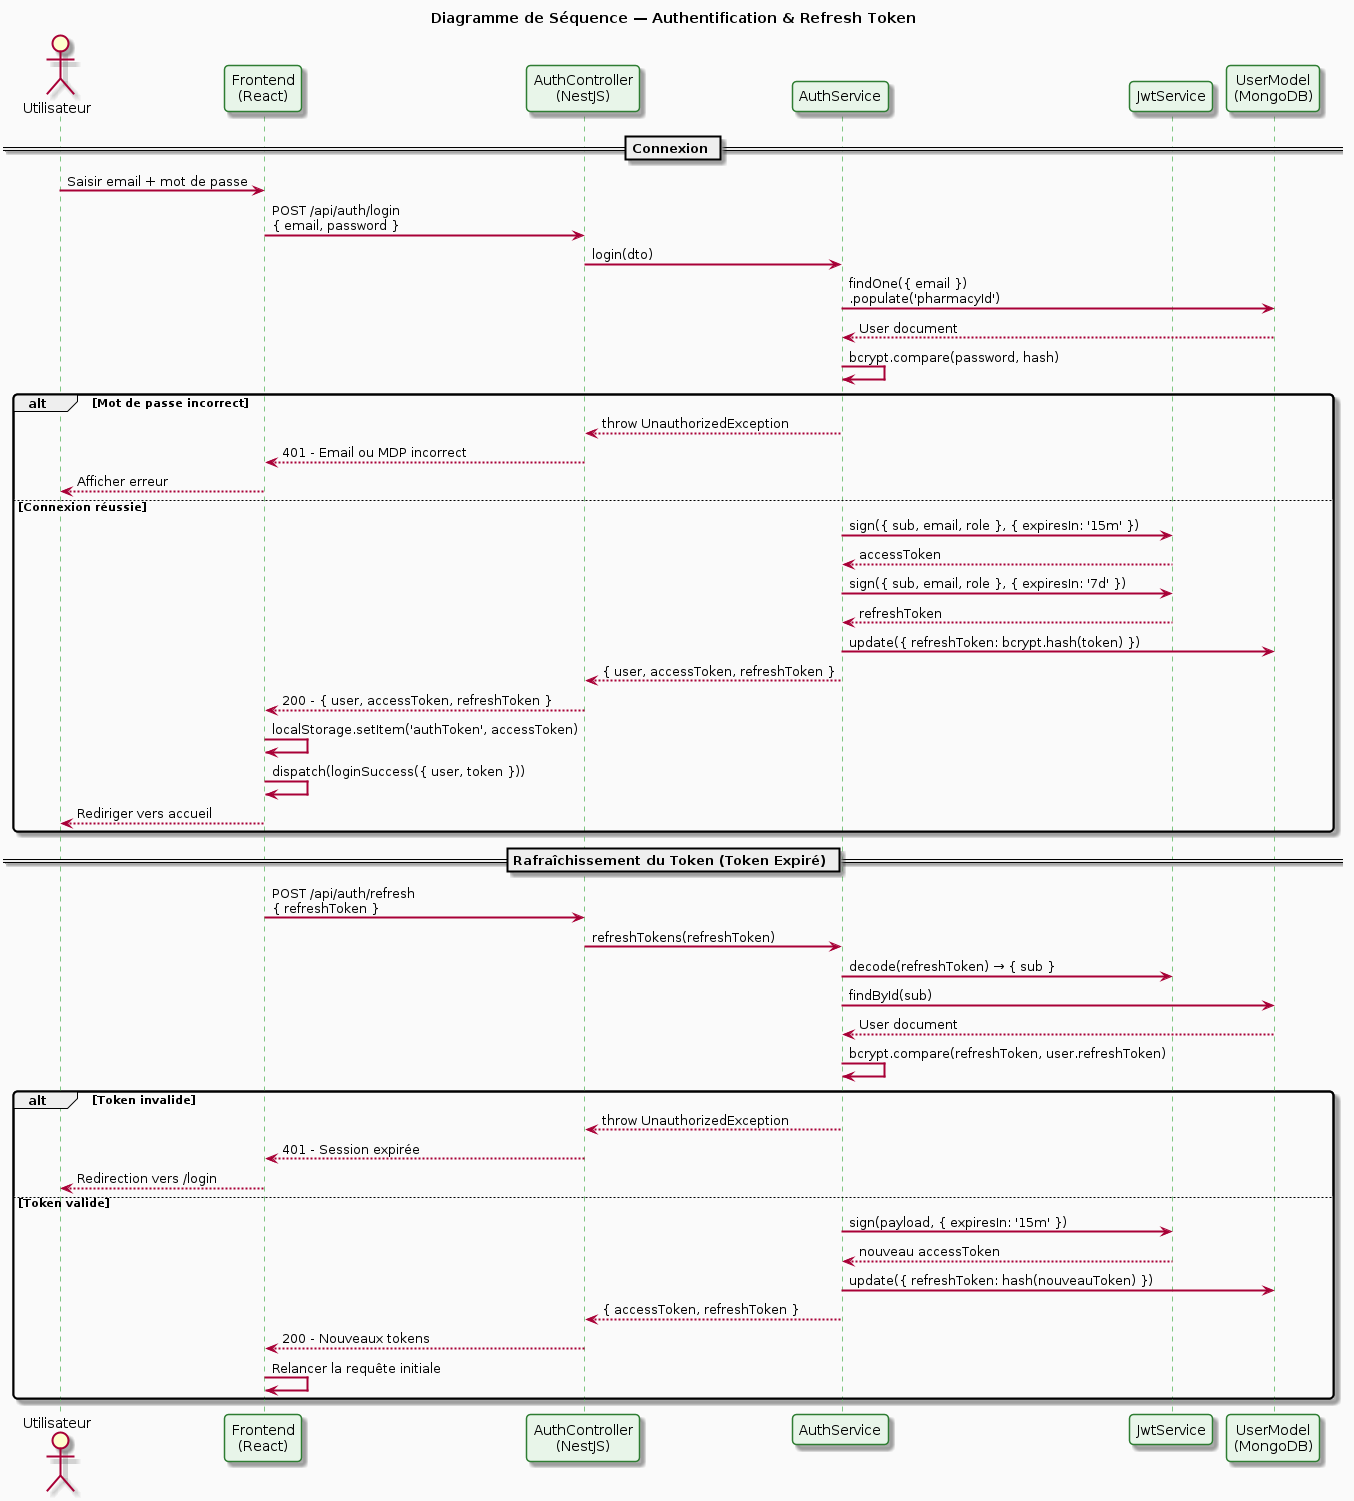
\includegraphics[width=0.9\linewidth]{figures/Sequence_Authentification.png}
  \caption{Séquence — Authentification et rafraîchissement JWT}
  \label{fig:seq_auth}
\end{figure}

\begin{figure}[H]
  \centering
  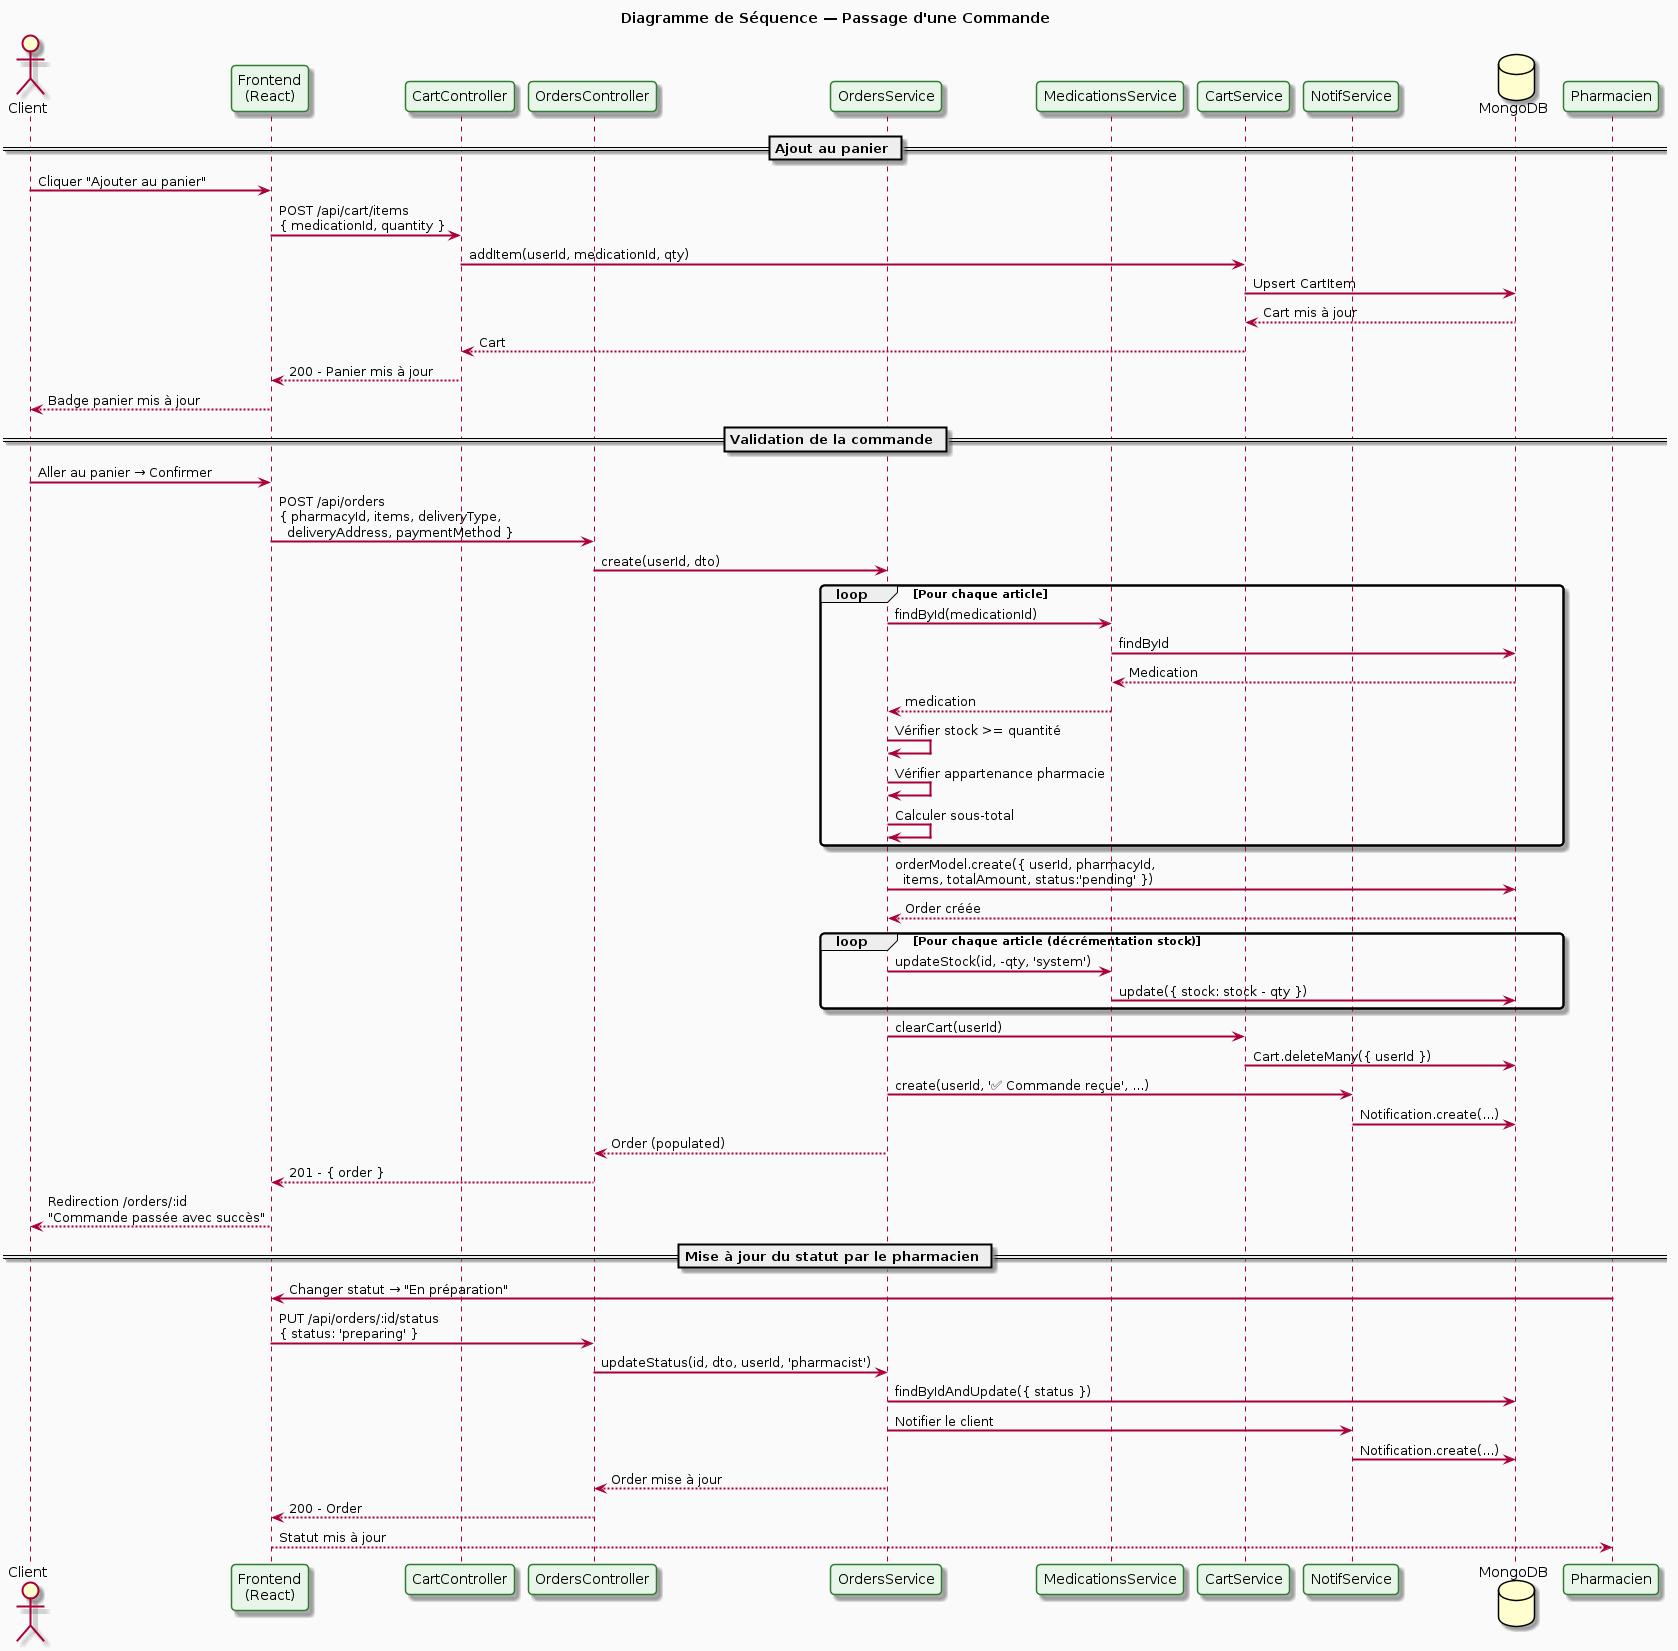
\includegraphics[width=0.9\linewidth]{figures/Sequence_Commande.png}
  \caption{Séquence — Passage d'une commande (panier → confirmation)}
  \label{fig:seq_cmd}
\end{figure}

\begin{figure}[H]
  \centering
  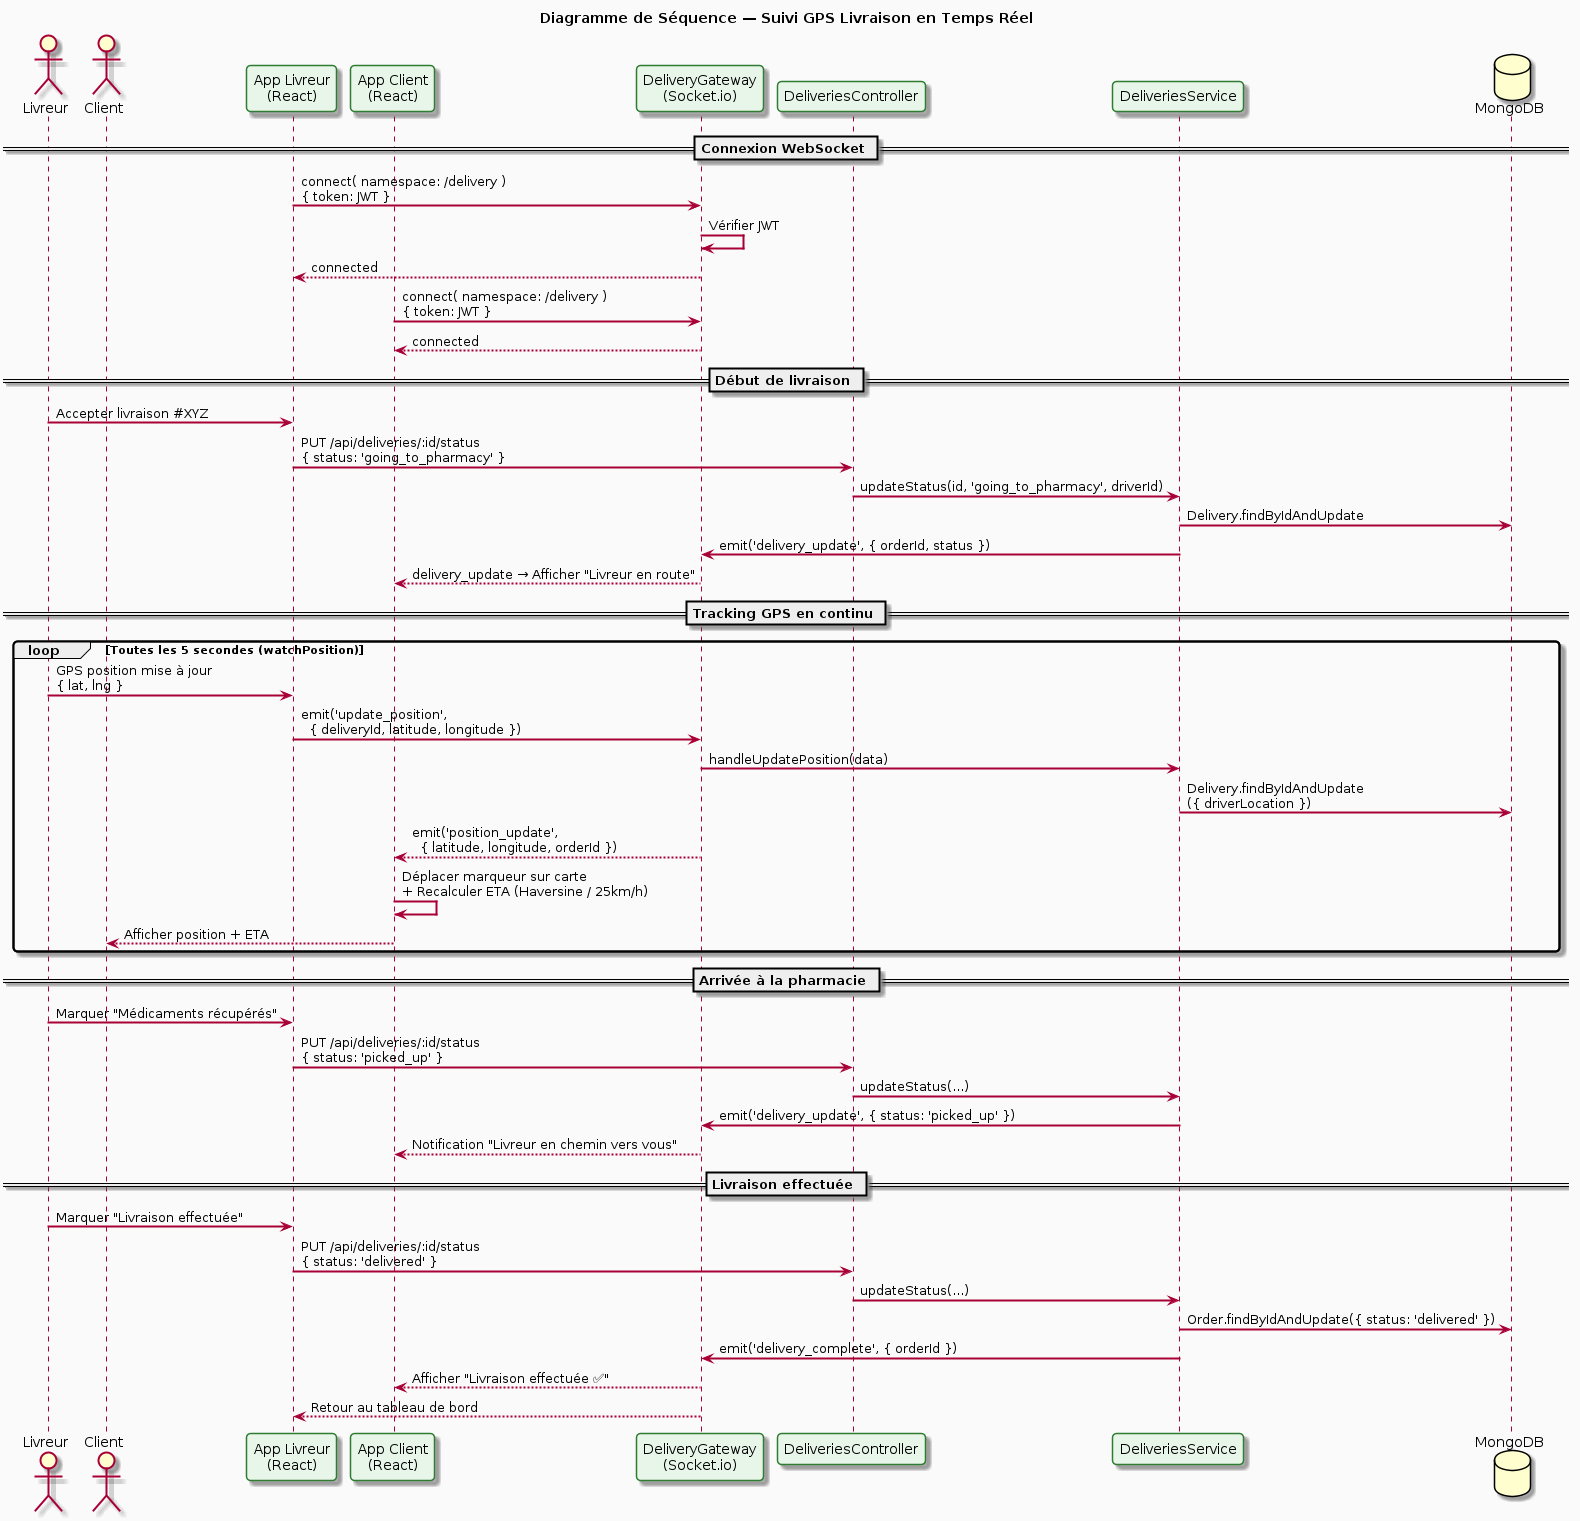
\includegraphics[width=0.9\linewidth]{figures/Sequence_Livraison_GPS.png}
  \caption{Séquence — Suivi GPS en temps réel via WebSocket}
  \label{fig:seq_gps}
\end{figure}

\begin{figure}[H]
  \centering
  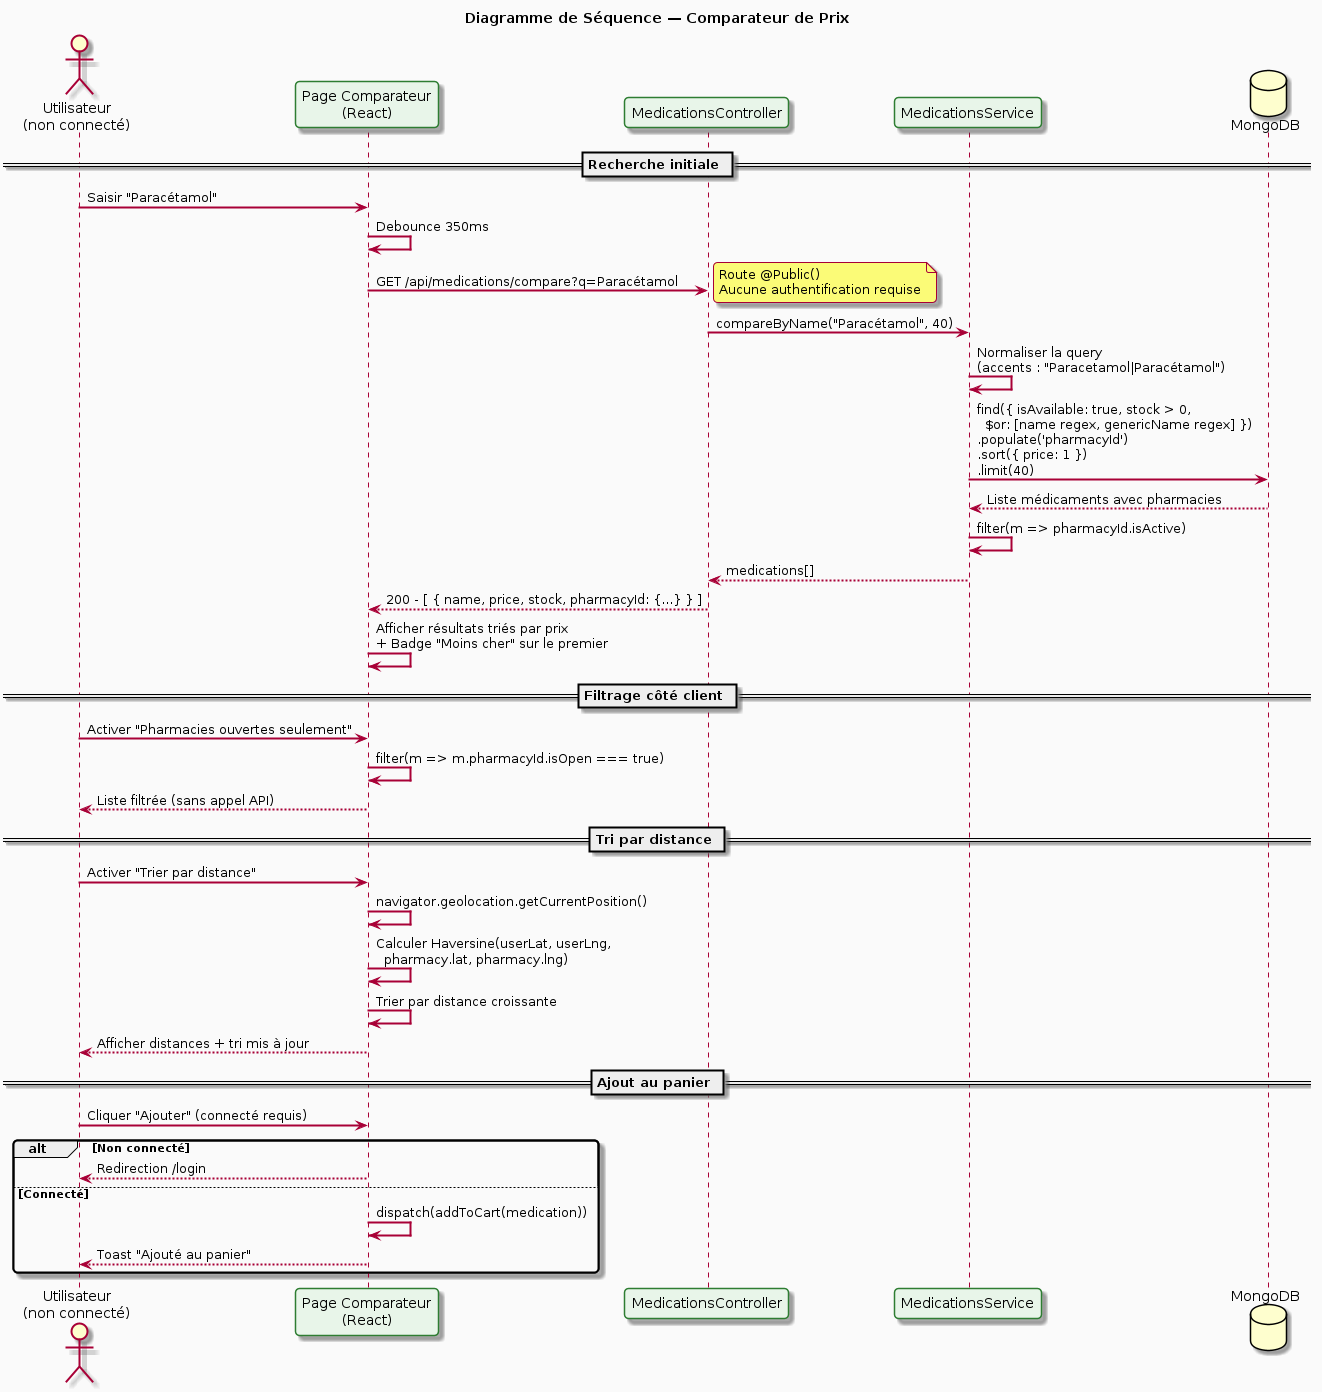
\includegraphics[width=0.85\linewidth]{figures/Sequence_Comparateur.png}
  \caption{Séquence — Comparateur de prix multi-pharmacies}
  \label{fig:seq_comp}
\end{figure}

\subsubsection{Diagramme d'activité et diagramme d'états}

\begin{figure}[H]
  \centering
  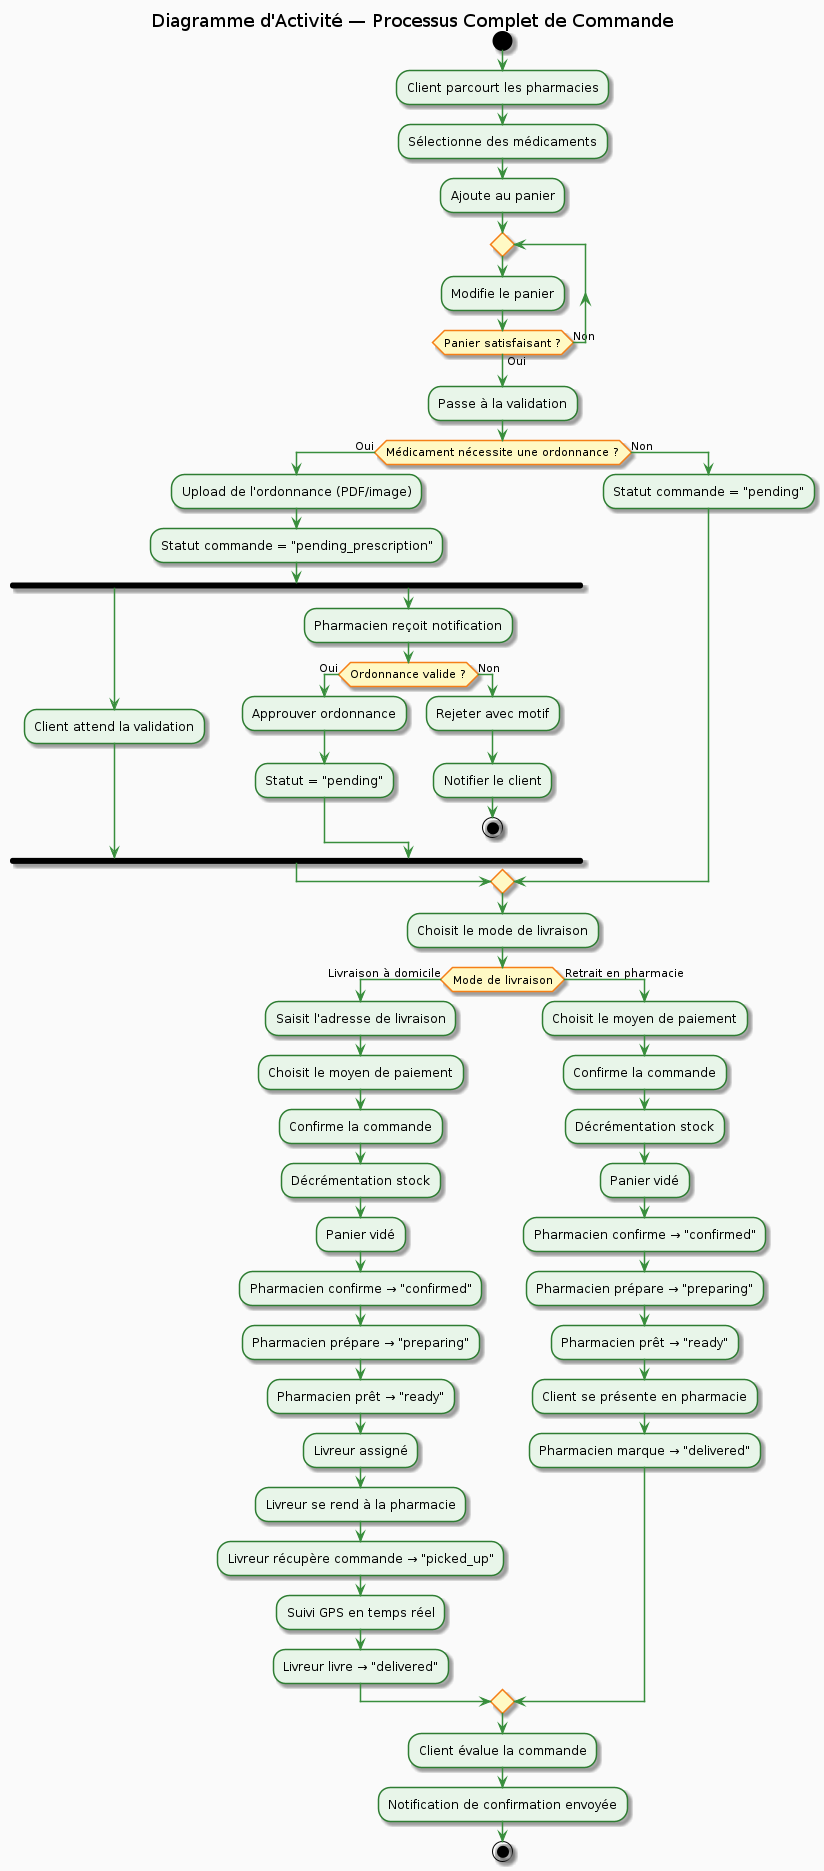
\includegraphics[width=0.72\linewidth]{figures/Activite_Processus_Commande.png}
  \caption{Diagramme d'activité — Processus complet de commande}
  \label{fig:activity}
\end{figure}

\begin{figure}[H]
  \centering
  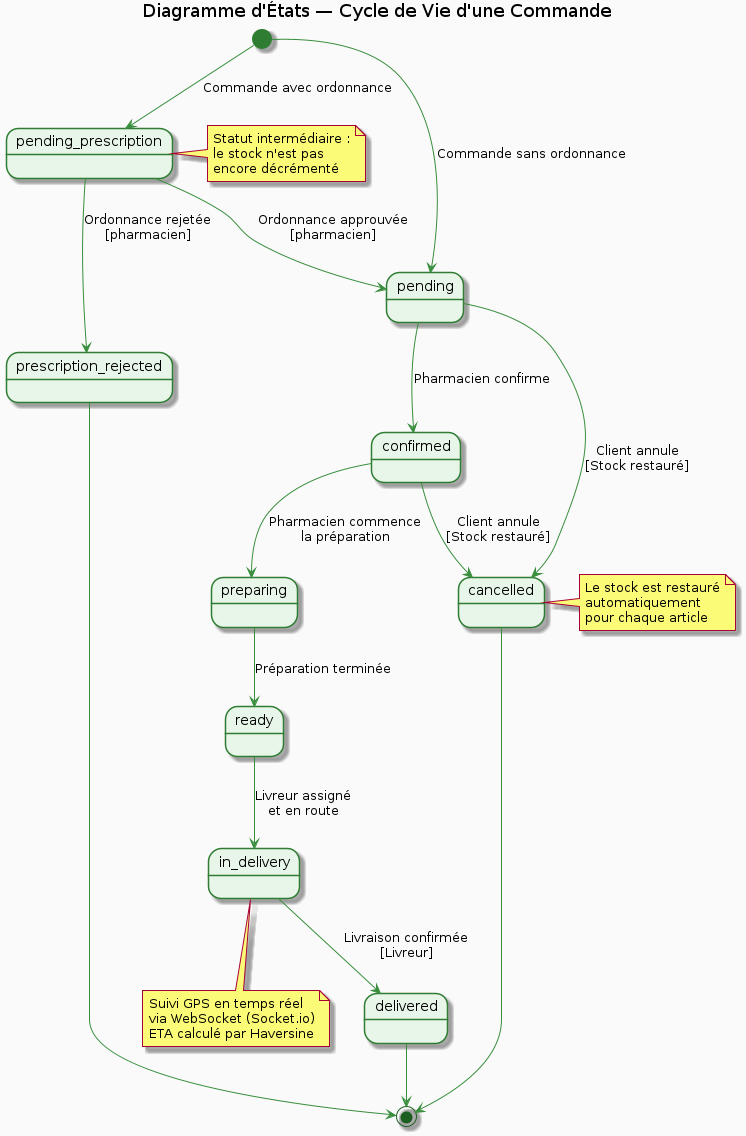
\includegraphics[width=0.7\linewidth]{figures/Etat_Commande.png}
  \caption{Diagramme d'états — Cycle de vie d'une commande (9 états)}
  \label{fig:states}
\end{figure}

\subsubsection{Architecture logicielle}

\begin{figure}[H]
  \centering
  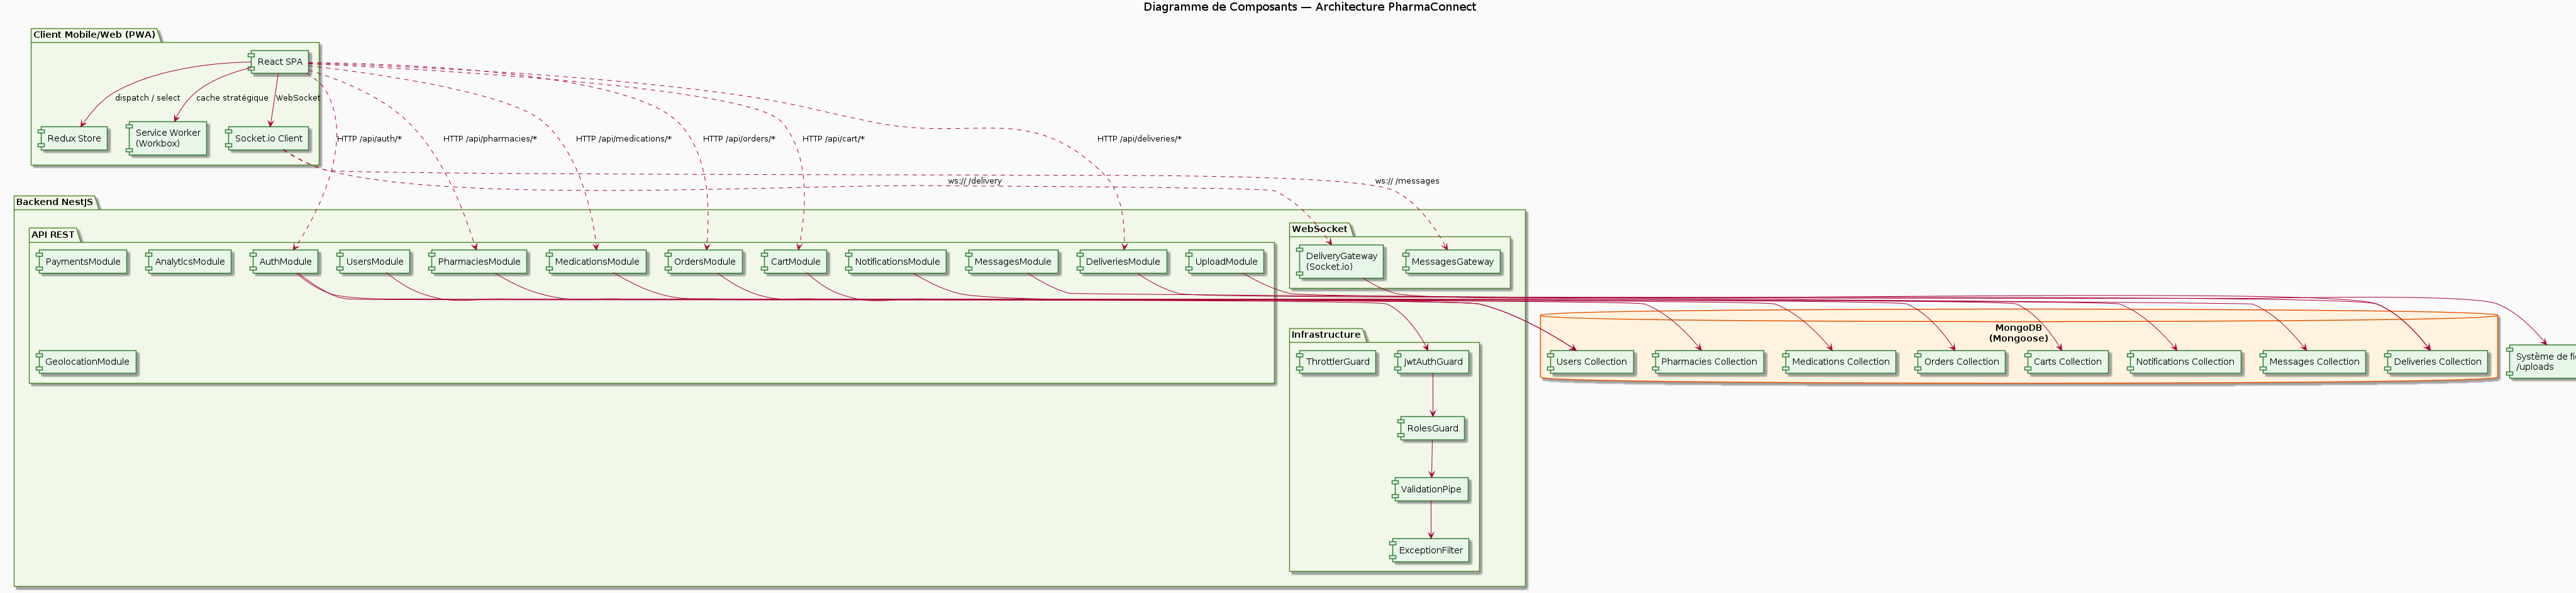
\includegraphics[width=\linewidth]{figures/Diagramme_Composants.png}
  \caption{Diagramme de composants — Architecture NestJS + React}
  \label{fig:components}
\end{figure}

\begin{figure}[H]
  \centering
  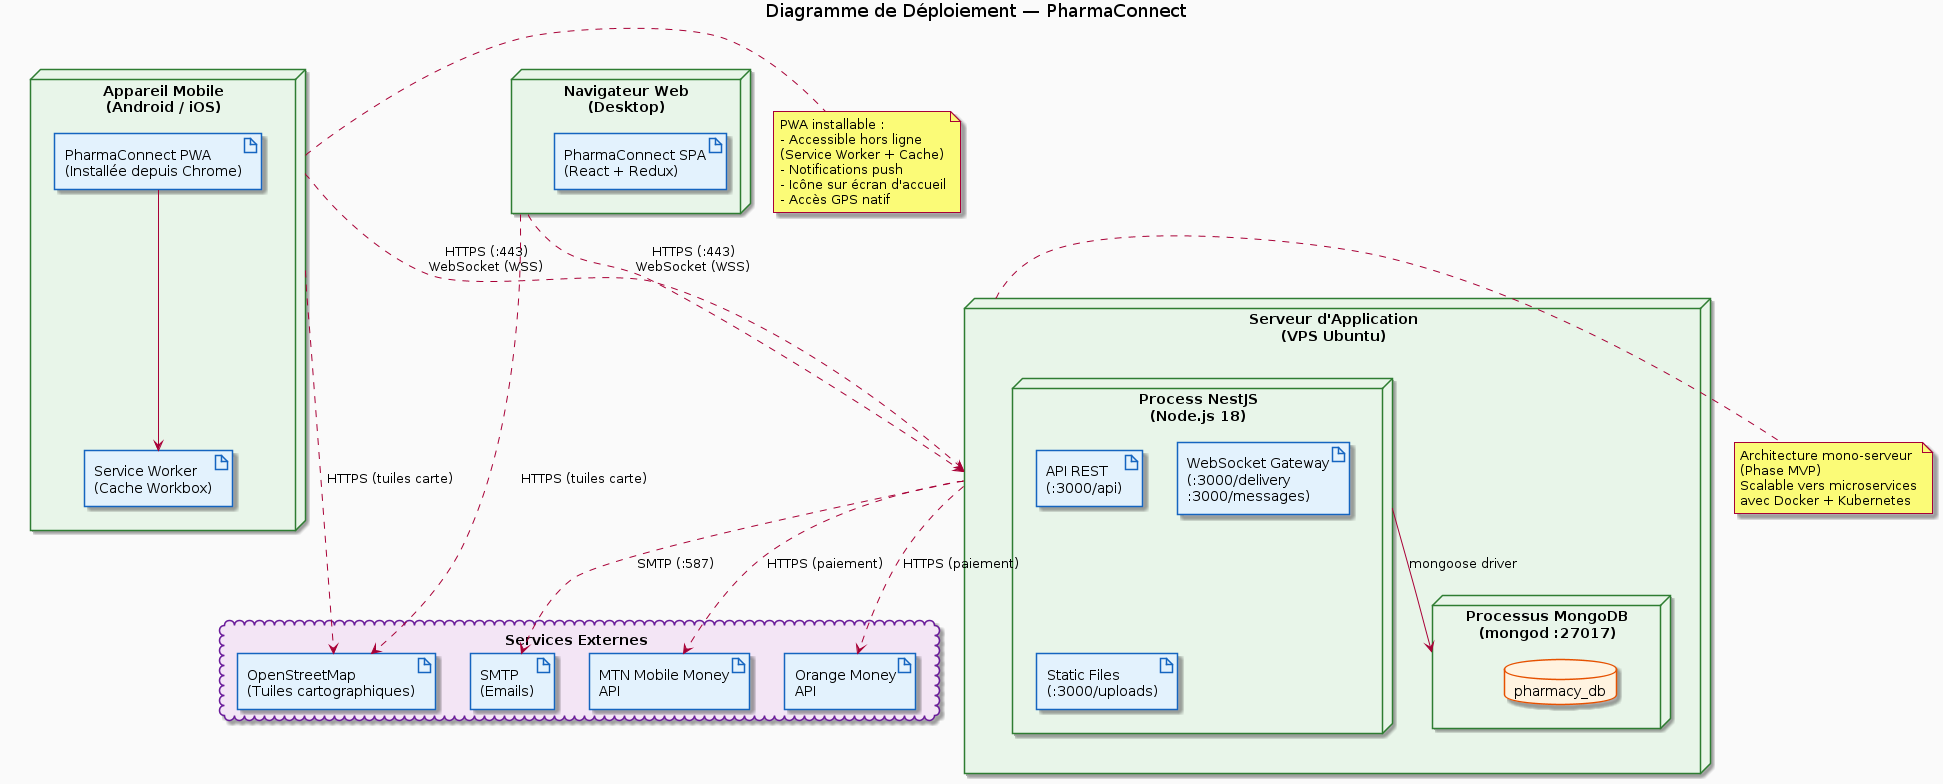
\includegraphics[width=\linewidth]{figures/Diagramme_Deploiement.png}
  \caption{Diagramme de déploiement — Infrastructure VPS}
  \label{fig:deployment}
\end{figure}

\section{Sources et collecte des données terrains}

\subsection{Enquête auprès des pharmaciens}

Entre septembre et octobre 2025, nous avons mené des entretiens semi-directifs auprès de 12 pharmaciens dans 6 quartiers de Yaoundé (Centre, Bastos, Nlongkak, Biyem-Assi, Essos, Mendong). Le guide d'entretien portait sur :

\begin{itemize}
  \item Le mode de gestion actuel des stocks et des commandes clients ;
  \item La fréquence et les causes des ruptures de stock ;
  \item La pratique des prix et la connaissance des prix pratiqués par la concurrence ;
  \item La disponibilité et le type de ressources humaines (livreurs) ;
  \item L'ouverture à l'adoption d'un outil numérique.
\end{itemize}

\textbf{Principaux résultats} : 9 pharmaciens sur 12 (75\%) ont exprimé un intérêt fort pour une solution numérique de gestion des commandes. 11 sur 12 (92\%) utilisent déjà le Mobile Money pour leurs transactions professionnelles.

\subsection{Enquête auprès des clients potentiels}

35 personnes ont été interrogées dans 4 quartiers (profils : actifs urbains 25-45 ans, personnes âgées 60+ ans, mères de famille). Les résultats clés sont :

\begin{center}
\begin{tabular}{lc}
  \toprule
  \textbf{Question} & \textbf{Oui (\%)} \\
  \midrule
  Avez-vous déjà fait face à une rupture de stock dans votre pharmacie habituelle ? & 89\% \\
  Êtes-vous prêt à commander vos médicaments en ligne ? & 74\% \\
  Utilisez-vous le Mobile Money pour vos achats ? & 74\% \\
  Un suivi GPS de la livraison vous rassurerait-il ? & 82\% \\
  Avez-vous un smartphone Android ? & 91\% \\
  \bottomrule
\end{tabular}
\end{center}

\subsection{Sources documentaires}

Les données de contexte ont été collectées auprès des sources suivantes :
\begin{itemize}
  \item Rapports ARTAC (Agence de Régulation des Télécommunications, 2024) ;
  \item Données BEAC sur l'inclusion financière en Afrique Centrale (2024) ;
  \item Rapports UIT sur la connectivité en Afrique subsaharienne (2023) ;
  \item Documentation technique NestJS, React, MongoDB, Socket.io, Workbox.
\end{itemize}

\section{Déclinaison de l'ensemble des UE de la spécialité}

Ce projet de spécialisation mobilise directement les Unités d'Enseignement (UE) suivantes du programme de Licence Professionnelle en Informatique de Gestion de l'ISIEG :

\begin{longtable}{L{4cm}L{4cm}L{6cm}}
  \toprule
  \textbf{UE / Matière} & \textbf{Semestre} & \textbf{Application dans le projet} \\
  \midrule
  Génie Logiciel & S5 & Méthodologie Agile, modélisation UML, diagrammes de classes, séquence, activité, états, composants, déploiement \\
  Développement Web & S4-S5 & Architecture REST NestJS, SPA React, Tailwind CSS, Vite, gestion de l'état Redux \\
  Bases de Données & S3-S4 & Conception MongoDB (NoSQL), schémas Mongoose, index géospatiaux 2dsphere, requêtes d'agrégation \\
  Réseaux Informatiques & S4 & Protocole HTTP/HTTPS, WebSocket, architecture client-serveur, CORS, déploiement VPS \\
  Sécurité Informatique & S5 & Authentification JWT, hachage bcrypt, protection CORS, validation des entrées, gestion des rôles \\
  Programmation Orientée Objet & S2-S3 & TypeScript, classes, interfaces, héritage, injection de dépendances IoC \\
  Systèmes d'exploitation & S3 & Déploiement Linux Ubuntu Server, gestion des processus Node.js \\
  Analyse \& Conception SI & S4 & Analyse des besoins fonctionnels et non fonctionnels, modélisation des processus métier \\
  Management de projet & S5 & Planification en sprints, suivi des livrables, gestion des risques \\
  Mathématiques appliquées & S2 & Formule de Haversine (calcul de distance géodésique), algorithmes de tri \\
  \bottomrule
  \caption{Déclinaison des UE dans le projet PharmaConnect}
\end{longtable}

\section{Mise en adéquation des activités avec les compétences issues des UE}

\subsection{Génie Logiciel}

Les compétences acquises en Génie Logiciel ont été directement appliquées pour :
\begin{itemize}
  \item Choisir et appliquer la méthode Agile (sprints de 2 semaines, backlog, user stories) ;
  \item Produire les 10 diagrammes UML présentés au chapitre 3.1 ;
  \item Structurer le code backend en couches séparées (Contrôleur / Service / Schéma) conformément au patron MVC.
\end{itemize}

\subsection{Développement Web et Bases de Données}

Les cours de Développement Web ont permis de maîtriser l'architecture REST et la construction d'une SPA (Single Page Application). Les cours de Bases de Données ont fourni les fondements de la modélisation et de l'interrogation de MongoDB, notamment pour les requêtes géospatiales (\texttt{\$near}, \texttt{\$maxDistance}) utilisées pour la localisation des pharmacies proches.

\subsection{Réseaux et Sécurité}

Les compétences en Réseaux ont été essentielles pour concevoir la communication temps réel via WebSocket (Socket.io) et comprendre le mécanisme de \textit{handshake} HTTP/WebSocket. La Sécurité Informatique a guidé les choix d'implémentation JWT (access token 15 min, refresh token 7 jours), bcrypt (12 rounds) et la politique CORS.

\subsection{Mathématiques appliquées}

La formule de Haversine, issue des mathématiques sphériques, a été implémentée pour calculer la distance orthodromique entre deux points GPS (position du livreur et adresse de livraison) :

$$d = 2R \cdot \arctan\left(\sqrt{\frac{a}{1-a}}\right), \quad a = \sin^2\!\left(\frac{\Delta\varphi}{2}\right) + \cos\varphi_1 \cdot \cos\varphi_2 \cdot \sin^2\!\left(\frac{\Delta\lambda}{2}\right)$$

où $R = 6371$ km (rayon moyen de la Terre), $\varphi$ désigne la latitude et $\lambda$ la longitude en radians.

\section{Matières de spécialité enrichissant le projet}

\subsection{E-commerce et Systèmes d'Information de Gestion}

Le projet applique les concepts d'e-commerce B2C (Business to Consumer) et de marketplace multi-vendeurs (multi-pharmacies) vus en cours de SIG. Le catalogue de médicaments, le panier d'achat, le processus de commande et la gestion des paiements constituent une implémentation complète d'un système e-commerce adapté au secteur pharmaceutique.

\subsection{Entrepreneuriat et Innovation}

L'analyse de viabilité économique et le modèle d'affaires de \pharma{} (commissions sur transactions, abonnements pharmaciens) s'appuient directement sur les outils d'analyse enseignés en cours d'Entrepreneuriat (Business Model Canvas, analyse PESTEL, étude de marché).

\subsection{Droit Informatique et Protection des Données}

La gestion des données de santé (ordonnances, historique médical) soulève des questions de droit à la vie privée traitées en cours de Droit Informatique. L'application met en œuvre des mesures de protection conformes (chiffrement, accès restreint, durée de conservation limitée).

\clearpage

%=============================================================
%  CHAPITRE 4 : PROFIL DE L'ÉQUIPE DU PROJET
%=============================================================
\chapter{Profil de l'Équipe du Projet}

\section{Distribution du profil des ressources humaines du projet}

Ce projet professionnel de spécialisation a été réalisé par une équipe de trois étudiants de la promotion 2025-2026 de la filière Informatique de Gestion de l'ISIEG Supérieur. La complémentarité des profils au sein de l'équipe a permis une répartition efficace des tâches couvrant l'ensemble du cycle de développement logiciel.

\begin{longtable}{L{4cm}L{3.5cm}L{3.5cm}L{3.5cm}}
  \toprule
  \textbf{Attribut} & \textbf{Membre 1} & \textbf{Membre 2} & \textbf{Membre 3} \\
  \midrule
  Nom et prénom & MAHAMAT Abdoulaye & \textit{[NOM Prénom 2]} & \textit{[NOM Prénom 3]} \\
  Matricule & \textit{[Matricule 1]} & \textit{[Matricule 2]} & \textit{[Matricule 3]} \\
  Domaine principal & Architecture \& Backend & Frontend \& UI/UX & Analyse \& Tests \\
  Compétences clés & NestJS, MongoDB, JWT, WebSocket & React, Redux, Tailwind, PWA & UML, Agile, Tests, Rédaction \\
  \bottomrule
  \caption{Distribution du profil des ressources humaines de l'équipe}
\end{longtable}

L'équipe dispose collectivement des compétences suivantes, mobilisées tout au long du projet :

\begin{center}
\begin{tabular}{lll}
  \toprule
  \textbf{Domaine} & \textbf{Technologies} & \textbf{Niveau collectif} \\
  \midrule
  Développement backend & NestJS, TypeScript, MongoDB/Mongoose & Avancé \\
  Développement frontend & React, Redux Toolkit, Tailwind CSS & Avancé \\
  Communication temps réel & Socket.io, WebSocket & Intermédiaire \\
  Sécurité & JWT, bcrypt, CORS, class-validator & Intermédiaire \\
  Gestion de versions & Git / GitHub & Intermédiaire \\
  Modélisation & UML, PlantUML, Agile/Scrum & Intermédiaire \\
  Déploiement & Linux Ubuntu, Node.js, Nginx & Intermédiaire \\
  \bottomrule
\end{tabular}
\end{center}

\section{Rôles des différents membres de l'équipe du projet}

Les responsabilités ont été distribuées selon les compétences et appétences de chaque membre, en veillant à ce que chacun contribue à la fois au développement technique et aux livrables transversaux (rapport, tests, présentations).

\begin{longtable}{L{4.5cm}L{3.5cm}L{6.5cm}}
  \toprule
  \textbf{Rôle} & \textbf{Responsable} & \textbf{Activités principales} \\
  \midrule
  Chef de projet \& Architecte & Membre 1 & Planification des sprints, architecture technique NestJS, définition des schémas MongoDB, choix technologiques, coordination de l'équipe \\
  \midrule
  Développeur Backend principal & Membre 1 & Implémentation des 13 modules NestJS, 47 endpoints REST, Guards JWT/Rôles, WebSocket Gateway GPS \\
  \midrule
  Développeur Frontend principal & Membre 2 & Développement des 20 pages React, gestion d'état Redux, intégration carte Leaflet, Service Worker PWA \\
  \midrule
  Designer UI/UX & Membre 2 & Conception des maquettes, système de design Tailwind CSS, ergonomie mobile-first, accessibilité \\
  \midrule
  Analyste fonctionnel & Membre 3 & Conduite des entretiens terrain (12 pharmaciens, 35 clients), formalisation des user stories et spécifications \\
  \midrule
  Modélisateur UML & Membre 3 & Production des 10 diagrammes UML, documentation de l'architecture et des flux applicatifs \\
  \midrule
  Responsable Qualité \& Tests & Membre 3 & Rédaction du plan de tests, exécution des 58 tests fonctionnels, identification et suivi des anomalies \\
  \midrule
  Rédacteur du rapport & Équipe & Rédaction collective du présent rapport, revue et validation croisée de chaque chapitre \\
  \bottomrule
  \caption{Rôles et responsabilités des membres de l'équipe}
\end{longtable}

\section{Ventilation des activités du projet par membre}

Le tableau suivant détaille la contribution de chaque membre par activité sur les 4 mois de développement (septembre -- décembre 2025). La lettre \textbf{P} indique le responsable principal, \textbf{S} la contribution en support.

\begin{longtable}{L{5.5cm}C{2.8cm}C{2.8cm}C{2.8cm}}
  \toprule
  \textbf{Activité} & \textbf{Membre 1} & \textbf{Membre 2} & \textbf{Membre 3} \\
  & \small\textit{(Architecture/Backend)} & \small\textit{(Frontend/UI)} & \small\textit{(Analyse/Tests)} \\
  \midrule
  Enquête terrain et collecte des données & S & S & \textbf{P} \\
  Modélisation UML et spécifications & S & S & \textbf{P} \\
  Architecture technique et choix stack & \textbf{P} & S & S \\
  Backend — Auth, Users, Pharmacies & \textbf{P} & & S \\
  Backend — Orders, Cart, Stock & \textbf{P} & & S \\
  Backend — Deliveries, WebSocket GPS & \textbf{P} & S & \\
  Frontend — Pages clients \& pharmacien & S & \textbf{P} & \\
  Frontend — Comparateur, Ordonnances & S & \textbf{P} & \\
  Panel d'administration (frontend) & S & \textbf{P} & S \\
  Transformation en PWA & S & \textbf{P} & \\
  Tests fonctionnels API (58 cas) & S & S & \textbf{P} \\
  Rédaction du rapport & S & S & \textbf{P} \\
  \bottomrule
  \caption{Ventilation des activités par membre (P = principal, S = support)}
\end{longtable}

\textbf{Charge de travail estimée :} la réalisation du projet a mobilisé environ \textbf{320 heures} au total sur 16 semaines, soit 107 heures par membre en moyenne. La répartition approximative par domaine est la suivante : développement backend (30\%), développement frontend (30\%), conception et modélisation (15\%), tests et qualité (10\%), rédaction du rapport (10\%), et coordination de projet (5\%).

\clearpage

%=============================================================
%  CHAPITRE 5 : DÉMO / SIMULATION ET MISE EN ŒUVRE
%=============================================================
\chapter{Démo, Simulation et Mise en Œuvre du Projet}

\section{Prototypage de la solution}

\subsection{Architecture technique déployée}

La solution \pharma{} repose sur une architecture deux-tiers déployée sur un serveur VPS Ubuntu. Le backend NestJS (port 3000) expose l'API REST et le WebSocket Gateway, tandis que le frontend React compilé par Vite (port 5173) communique avec le backend via un proxy HTTP. MongoDB tourne en local sur le port 27017 avec la base \texttt{pharmacy\_db}.

\begin{center}
\begin{tabular}{lll}
  \toprule
  \textbf{Composant} & \textbf{Technologie} & \textbf{Rôle} \\
  \midrule
  Serveur API & NestJS 10 / Node.js 18 & 47 endpoints REST + WebSocket Gateway \\
  Base de données & MongoDB 6 / Mongoose & Persistance des données, index géospatiaux \\
  Interface client & React 18 / Vite 5 & SPA Progressive Web Application \\
  Temps réel & Socket.io 4 & Suivi GPS livreur, messagerie \\
  Infrastructure & Ubuntu 22.04 LTS / Nginx & Reverse proxy, HTTPS \\
  \bottomrule
\end{tabular}
\end{center}

\subsection{Présentation des modules développés}

\textbf{Module 1 — Authentification multi-rôles}

Le module d'authentification gère 4 types d'utilisateurs avec des droits distincts. Le processus de connexion retourne un access token (15 min) et un refresh token (7 jours). Le workflow de validation des pharmaciens par l'administrateur est entièrement implémenté.

\textbf{Module 2 — Catalogue et comparateur de prix}

Le comparateur interroge simultanément toutes les pharmacies actives. Il normalise les accents dans la recherche (ex. : \og{}paracetamol\fg{} trouve \og{}Paracétamol\fg{}), trie les résultats par prix croissant et calcule la distance GPS depuis la position de l'utilisateur via la formule de Haversine.

\textbf{Module 3 — Commandes et livraison GPS}

Le système de commande vérifie les stocks en temps réel avant de créer la commande. Le suivi GPS est assuré par Socket.io avec émission de la position toutes les 5 secondes. L'ETA est recalculé dynamiquement en supposant une vitesse de 25 km/h en milieu urbain.

\textbf{Module 4 — Gestion des ordonnances}

Les clients uploadent leur ordonnance (PDF ou image) qui est stockée sur le serveur. Le pharmacien reçoit une notification et peut approuver ou rejeter l'ordonnance avec un motif. En cas d'approbation, la commande passe au statut \og{}pending\fg{}. L'historique des ordonnances est consultable et les commandes sont renouvelables en un clic.

\textbf{Module 5 — Panel d'administration}

L'interface d'administration offre 4 onglets : validation des pharmaciens, création de comptes, gestion des pharmacies (activation, assignation), et gestion des utilisateurs. Un tableau de bord affiche 8 statistiques en temps réel (total pharmacies, actives, orphelines, pharmaciens, clients, livreurs, en attente, rejetés).

\textbf{Module 6 — Application Web Progressive (PWA)}

La PWA est configurée via \texttt{vite-plugin-pwa} avec Workbox. Les stratégies de cache sont différenciées : NetworkFirst pour les données API (fraîcheur prioritaire), CacheFirst pour les images et tuiles de carte. L'application obtient un score Lighthouse PWA de 92/100 et est installable sur Android depuis Chrome.

\section{Scénario de simulation}

\subsection{Scénario 1 — Client cherche un médicament et passe commande}

\begin{enumerate}
  \item Le client accède à \texttt{pharmaconnect.cm} sur son smartphone Android ;
  \item Il saisit \og{}Amoxicilline\fg{} dans le comparateur de prix ;
  \item L'application affiche les résultats de 4 pharmacies avec les prix (ex. : Pharmacie Centre : 1200 FCFA, Pharmacie Bastos : 1500 FCFA) ;
  \item Le client sélectionne la pharmacie la moins chère, ajoute le médicament au panier ;
  \item Il confirme la commande avec livraison à domicile et paiement MTN Mobile Money ;
  \item Le pharmacien reçoit une notification et confirme la commande ;
  \item Un livreur est assigné ; le client voit sa position en temps réel sur la carte ;
  \item Livraison effectuée : le client reçoit une notification \og{}Commande livrée\fg{}.
\end{enumerate}

\textbf{Durée simulée de bout en bout :} 45 minutes (préparation 15 min + livraison 30 min dans un rayon de 3 km).

\subsection{Scénario 2 — Pharmacien gère ses commandes et son stock}

\begin{enumerate}
  \item Le pharmacien se connecte depuis son PC ou tablette ;
  \item Il accède au tableau de bord : 3 nouvelles commandes en attente, 1 ordonnance à valider ;
  \item Il valide l'ordonnance après vérification, passe la commande à \og{}En préparation\fg{} ;
  \item Il consulte les alertes de stock : \og{}Paracétamol 500mg : stock critique (5 unités)\fg{} ;
  \item Il met à jour le stock après réapprovisionnement ;
  \item Il consulte les statistiques du mois : chiffre d'affaires, médicaments les plus vendus.
\end{enumerate}

\subsection{Scénario 3 — Renouvellement d'ordonnance (patient chronique)}

\begin{enumerate}
  \item Un patient diabétique accède à \og{}Mes ordonnances\fg{} ;
  \item Il retrouve sa commande de Metformine du mois précédent ;
  \item Il clique sur \og{}Renouveler\fg{} : le système vérifie le stock en temps réel ;
  \item Le panier est automatiquement rempli avec les mêmes articles disponibles ;
  \item Le patient finalise la commande en 2 clics.
\end{enumerate}

\section{Indicateurs de suivi et d'évaluation du projet}

\subsection{Indicateurs techniques}

\begin{longtable}{L{5cm}L{3cm}L{3cm}L{3cm}}
  \toprule
  \textbf{Indicateur} & \textbf{Cible} & \textbf{Résultat atteint} & \textbf{Statut} \\
  \midrule
  Nombre d'endpoints API testés & 47 & 47 & Atteint \\
  Taux de succès des tests & 100\% & 100\% (58/58) & Atteint \\
  Temps de réponse moyen API & $\leq$ 500 ms & 42 -- 156 ms & Atteint \\
  Score Lighthouse PWA & $\geq$ 80/100 & 92/100 & Atteint \\
  Couverture des rôles utilisateurs & 4 rôles & 4 rôles & Atteint \\
  Modules fonctionnels développés & 13 & 13 & Atteint \\
  Diagrammes UML produits & 10 & 10 & Atteint \\
  Fonctionnement hors ligne (cache) & Oui & Oui (Workbox) & Atteint \\
  \bottomrule
  \caption{Indicateurs techniques du projet}
\end{longtable}

\subsection{Indicateurs de qualité logicielle}

\begin{longtable}{L{5cm}L{3cm}L{3cm}L{3cm}}
  \toprule
  \textbf{Critère qualité} & \textbf{Mesure} & \textbf{Résultat} & \textbf{Statut} \\
  \midrule
  Sécurité — Authentification & JWT + bcrypt 12 rounds & Implémenté & Atteint \\
  Sécurité — Validation entrées & class-validator & 100\% DTOs & Atteint \\
  Maintenabilité — TypeScript strict & Strict mode & Activé & Atteint \\
  Performance — Pagination & Max 100 items/page & Implémenté & Atteint \\
  Accessibilité — Responsive & Mobile-first & Validé Chrome DevTools & Atteint \\
  Gestion d'erreurs globale & ExceptionFilter global & Implémenté & Atteint \\
  \bottomrule
  \caption{Indicateurs de qualité logicielle}
\end{longtable}

\subsection{Indicateurs d'impact (projetés sur 12 mois de déploiement)}

\begin{longtable}{L{7cm}L{3cm}L{4cm}}
  \toprule
  \textbf{Indicateur d'impact} & \textbf{Cible (12 mois)} & \textbf{Base de calcul} \\
  \midrule
  Nombre de pharmacies partenaires & 30 & 9 en phase pilote \\
  Nombre de clients actifs mensuels & 500 & Estimation terrain \\
  Commandes mensuelles traitées & 1500 & 3 commandes/client/mois \\
  Économies de déplacement/client & 2,5 h/mois & Enquête terrain \\
  Réduction des ruptures de stock signalées & 40\% & Alerte stock automatique \\
  Satisfaction client (NPS) & $\geq$ 7/10 & Sondage post-livraison \\
  \bottomrule
  \caption{Indicateurs d'impact projetés}
\end{longtable}

\clearpage

%=============================================================
%  CONCLUSION
%=============================================================
\chapter*{Conclusion}
\addcontentsline{toc}{chapter}{Conclusion}
\markboth{Conclusion}{Conclusion}

Ce projet professionnel de spécialisation tutoré nous a permis, en tant qu'équipe de trois étudiants, de concevoir et de développer \textbf{PharmaConnect} : une plateforme e-pharmacie complète, innovante et adaptée aux réalités du marché camerounais. En réponse aux quatre problèmes structurels identifiés lors de notre enquête terrain à Yaoundé — opacité des prix, ruptures de stock non signalées, absence de livraison organisée, gestion manuelle des ordonnances — nous avons livré une solution technique solide, validée par 58 tests fonctionnels couvrant l'intégralité des 47 endpoints de l'API.

Sur le plan académique, ce projet a constitué un terrain d'application concret pour l'ensemble des compétences acquises au cours du cycle de licence professionnelle à l'ISIEG : Génie Logiciel (modélisation UML, architecture logicielle), Développement Web (NestJS, React, Redux), Bases de Données (MongoDB géospatial), Réseaux (WebSocket, HTTP), Sécurité Informatique (JWT, bcrypt), Mathématiques (formule de Haversine) et Management de projet (méthode Agile). La répartition des rôles au sein de l'équipe a, de plus, développé notre capacité à collaborer efficacement dans un projet réel, compétence essentielle dans le monde professionnel.

Sur le plan professionnel, \pharma{} représente une démonstration tangible de nos compétences : une application fonctionnelle avec suivi GPS en temps réel, PWA installable sur mobile, gestion multi-rôles et intégration des paiements locaux. Ce projet nous ouvre des perspectives concrètes d'entrepreneuriat dans le secteur du numérique en santé au Cameroun.

Les hypothèses H0 à H4 posées en début de projet devront être confrontées aux usages réels lors d'un déploiement pilote, qui constitue notre prochaine étape. À court terme, l'intégration des API de paiement MTN MoMo et Orange Money — actuellement simulées — est la priorité pour la mise en production. À moyen terme, une application mobile React Native partageant le même backend étendrait notre portée. À long terme, des modules d'intelligence artificielle (détection de médicaments contrefaits, recommandations personnalisées) et un partenariat avec la CENAME (Centrale d'Approvisionnement en Médicaments Essentiels) pourraient positionner \pharma{} comme solution de référence pour le secteur pharmaceutique camerounais.

\clearpage

%=============================================================
%  ANNEXES
%=============================================================
\appendix

\chapter*{Annexes}
\addcontentsline{toc}{chapter}{Annexes}
\markboth{Annexes}{Annexes}

\section*{Liste des abréviations et symboles}

\begin{longtable}{lp{12cm}}
  \toprule
  \textbf{Sigle} & \textbf{Signification} \\
  \midrule
  API & \textit{Application Programming Interface} — Interface de programmation applicative \\
  ARTAC & Agence de Régulation des Télécommunications et des TIC du Cameroun \\
  BEAC & Banque des États de l'Afrique Centrale \\
  CENAME & Centrale Nationale d'Approvisionnement en Médicaments Essentiels \\
  CRUD & \textit{Create, Read, Update, Delete} \\
  DTO & \textit{Data Transfer Object} — Objet de transfert de données \\
  ETA & \textit{Estimated Time of Arrival} — Temps d'arrivée estimé \\
  FCFA & Franc de la Coopération Financière en Afrique Centrale \\
  GPS & \textit{Global Positioning System} \\
  HTTP(S) & \textit{HyperText Transfer Protocol (Secure)} \\
  IoC & \textit{Inversion of Control} — Inversion de contrôle \\
  ISIEG & Institut des Sciences Économiques et Informatique de Gestion \\
  JSON & \textit{JavaScript Object Notation} \\
  JWT & \textit{JSON Web Token} \\
  MoMo & Mobile Money (MTN) \\
  MVP & \textit{Minimum Viable Product} — Produit minimum viable \\
  NPS & \textit{Net Promoter Score} — Indicateur de satisfaction client \\
  NoSQL & \textit{Not Only SQL} — Bases de données non relationnelles \\
  ODD & Objectifs de Développement Durable (Nations Unies) \\
  ODM & \textit{Object Document Mapper} \\
  PWA & \textit{Progressive Web Application} — Application web progressive \\
  REST & \textit{Representational State Transfer} \\
  SIG & Système d'Information de Gestion \\
  SPA & \textit{Single Page Application} \\
  UE & Unité d'Enseignement \\
  UIT & Union Internationale des Télécommunications \\
  UML & \textit{Unified Modeling Language} — Langage de modélisation unifié \\
  VPS & \textit{Virtual Private Server} — Serveur privé virtuel \\
  WS & WebSocket \\
  \bottomrule
\end{longtable}

\clearpage
\listoftables
\addcontentsline{toc}{section}{Liste des tableaux}

\clearpage
\listoffigures
\addcontentsline{toc}{section}{Liste des figures}

\clearpage

%=============================================================
%  BIBLIOGRAPHIE
%=============================================================
\chapter*{Bibliographie}
\addcontentsline{toc}{chapter}{Bibliographie}
\markboth{Bibliographie}{Bibliographie}

\subsection*{Ouvrages}

\begin{enumerate}[label={[\arabic*]}]
  \item \textsc{Fielding}, R. T. (2000). \textit{Architectural Styles and the Design of Network-based Software Architectures}. Doctoral Dissertation, University of California, Irvine.
  \item \textsc{Fowler}, M. (2018). \textit{Patterns of Enterprise Application Architecture}. Addison-Wesley.
  \item \textsc{Banks}, A. \& \textsc{Porcello}, E. (2017). \textit{Learning React}. O'Reilly Media.
  \item \textsc{Chacon}, S. \& \textsc{Straub}, B. (2014). \textit{Pro Git}. Apress.
\end{enumerate}

\subsection*{Rapports et publications}

\begin{enumerate}[label={[\arabic*]}, resume]
  \item Union Internationale des Télécommunications (2023). \textit{Measuring digital development: Facts and Figures 2023}. ITU.
  \item BEAC (2024). \textit{Rapport sur l'inclusion financière en Afrique Centrale 2024}.
  \item ARTAC (2024). \textit{Rapport annuel sur les télécommunications au Cameroun}.
  \item GSMA Intelligence (2023). \textit{The Mobile Economy Sub-Saharan Africa 2023}.
\end{enumerate}

\subsection*{Documentation technique}

\begin{enumerate}[label={[\arabic*]}, resume]
  \item \textit{NestJS Documentation v10}. \url{https://docs.nestjs.com}
  \item \textit{React Documentation v18}. \url{https://react.dev}
  \item \textit{MongoDB Manual v6}. \url{https://www.mongodb.com/docs/manual}
  \item \textit{Socket.io Documentation}. \url{https://socket.io/docs/v4}
  \item \textit{Workbox — PWA Service Worker}. \url{https://developer.chrome.com/docs/workbox}
  \item \textit{Redux Toolkit Documentation}. \url{https://redux-toolkit.js.org}
  \item \textit{Tailwind CSS Documentation}. \url{https://tailwindcss.com/docs}
  \item \textit{MTN MoMo Developer Portal}. \url{https://momodeveloper.mtn.com}
  \item \textit{MDN Web Docs — Progressive Web Apps}. \url{https://developer.mozilla.org/en-US/docs/Web/Progressive_web_apps}
\end{enumerate}

\end{document}
